\documentclass[11pt]{article}
% =======================================================================
%   Shared style for CS 300 notes.
%   Usage: place `% =======================================================================
%   Shared style for CS 300 notes.
%   Usage: place `% =======================================================================
%   Shared style for CS 300 notes.
%   Usage: place `\input{../../notes-style.tex}` right after \documentclass
%   in each chapter's lectures.tex and notes.tex.
% =======================================================================

% ---- Layout -----------------------------------------------------------
\usepackage[margin=1in]{geometry}
\usepackage{parskip}        % space between paragraphs, no indent
\usepackage{microtype}      % subtle kerning/spacing improvements

% ---- Colors (muted palette, easy on light-sensitive eyes) -------------
\usepackage{xcolor}
\definecolor{pagebg}       {HTML}{FAF6F0}  % warm cream background
\definecolor{bodyfg}       {HTML}{3D3A36}  % warm dark gray body text
\definecolor{heading}      {HTML}{3D6A6B}  % muted teal
\definecolor{subheading}   {HTML}{5B7A9C}  % dusty blue
\definecolor{accent}       {HTML}{8A6B4A}  % warm tan
\definecolor{linkcol}      {HTML}{5B7A9C}  % same as subheading
\definecolor{mutedtext}    {HTML}{6B6560}  % secondary / caption text
\definecolor{rulecol}      {HTML}{C8BFB0}  % separator / rule

% Callout box palette
\definecolor{defnFrame}    {HTML}{9DB89B}  \definecolor{defnBack}    {HTML}{EEF2E8}
\definecolor{ideaFrame}    {HTML}{9FB4CD}  \definecolor{ideaBack}    {HTML}{E8EEF5}
\definecolor{warnFrame}    {HTML}{CFAE87}  \definecolor{warnBack}    {HTML}{F5EDDF}
\definecolor{noteFrame}    {HTML}{BFA6AE}  \definecolor{noteBack}    {HTML}{F2E8EE}
\definecolor{exFrame}      {HTML}{9FBDBD}  \definecolor{exBack}      {HTML}{E8F0F0}
\definecolor{codeBack}     {HTML}{F3EDE2}
\definecolor{codeBorder}   {HTML}{D4CBBA}
\definecolor{codeKeyword}  {HTML}{6B4F7A}
\definecolor{codeString}   {HTML}{8A6B4A}
\definecolor{codeComment}  {HTML}{8A857F}

% ---- Page background + base text color --------------------------------
\usepackage{pagecolor}
\pagecolor{pagebg}
\color{bodyfg}

% ---- Fonts ------------------------------------------------------------
\usepackage[T1]{fontenc}
\IfFileExists{libertine.sty}{%
    \usepackage{libertine}      % warm, readable serif
    \usepackage[scaled=0.95]{inconsolata}  % softer monospace
}{}

% ---- Hyperref ---------------------------------------------------------
\usepackage{hyperref}
\hypersetup{
    colorlinks=true,
    linkcolor=linkcol,
    urlcolor=linkcol,
    citecolor=linkcol,
    pdfborder={0 0 0},
}

% ---- Section styling --------------------------------------------------
\usepackage[explicit]{titlesec}
\titleformat{\section}
    {\color{heading}\Large\bfseries}
    {\color{heading}\thesection\hspace{0.6em}}{0pt}{#1}
\titleformat{\subsection}
    {\color{subheading}\large\bfseries}
    {\color{subheading}\thesubsection\hspace{0.5em}}{0pt}{#1}
\titleformat{\subsubsection}
    {\color{accent}\normalsize\bfseries}
    {\color{accent}\thesubsubsection\hspace{0.5em}}{0pt}{#1}
\titleformat{\paragraph}[runin]
    {\color{accent}\bfseries}{}{0pt}{#1.}

\titlespacing*{\section}{0pt}{1.6em}{0.6em}
\titlespacing*{\subsection}{0pt}{1.2em}{0.4em}

% ---- Enumerate / itemize spacing --------------------------------------
\usepackage{enumitem}
\setlist[itemize]{leftmargin=1.4em, itemsep=2pt, topsep=4pt}
\setlist[enumerate]{leftmargin=1.6em, itemsep=2pt, topsep=4pt}

% ---- Code listings ----------------------------------------------------
\usepackage{listings}
\lstdefinestyle{notescode}{
    backgroundcolor=\color{codeBack},
    basicstyle=\ttfamily\small\color{bodyfg},
    keywordstyle=\color{codeKeyword}\bfseries,
    stringstyle=\color{codeString},
    commentstyle=\color{codeComment}\itshape,
    frame=single,
    framesep=6pt,
    rulecolor=\color{codeBorder},
    showstringspaces=false,
    breaklines=true,
    xleftmargin=10pt,
    xrightmargin=10pt,
    aboveskip=8pt,
    belowskip=8pt,
}
\lstset{style=notescode}

% ---- Callout boxes (tcolorbox) ----------------------------------------
\usepackage[most]{tcolorbox}

\newtcolorbox{defnbox}[1][]{
    enhanced, breakable,
    colback=defnBack, colframe=defnFrame, coltitle=bodyfg,
    title={\bfseries Definition \textemdash\ #1},
    fonttitle=\bfseries,
    boxrule=0.5pt, arc=2pt, left=8pt, right=8pt, top=6pt, bottom=6pt,
    attach boxed title to top left={xshift=10pt, yshift=-6pt},
    boxed title style={colback=defnFrame, colframe=defnFrame, arc=2pt},
    before skip=8pt, after skip=8pt,
}
\newtcolorbox{ideabox}[1][]{
    enhanced, breakable,
    colback=ideaBack, colframe=ideaFrame, coltitle=bodyfg,
    title={\bfseries Key idea #1},
    boxrule=0.5pt, arc=2pt, left=8pt, right=8pt, top=6pt, bottom=6pt,
    attach boxed title to top left={xshift=10pt, yshift=-6pt},
    boxed title style={colback=ideaFrame, colframe=ideaFrame, arc=2pt},
    before skip=8pt, after skip=8pt,
}
\newtcolorbox{warnbox}[1][]{
    enhanced, breakable,
    colback=warnBack, colframe=warnFrame, coltitle=bodyfg,
    title={\bfseries Gotcha #1},
    boxrule=0.5pt, arc=2pt, left=8pt, right=8pt, top=6pt, bottom=6pt,
    attach boxed title to top left={xshift=10pt, yshift=-6pt},
    boxed title style={colback=warnFrame, colframe=warnFrame, arc=2pt},
    before skip=8pt, after skip=8pt,
}
\newtcolorbox{notebox}[1][]{
    enhanced, breakable,
    colback=noteBack, colframe=noteFrame, coltitle=bodyfg,
    title={\bfseries Aside #1},
    boxrule=0.5pt, arc=2pt, left=8pt, right=8pt, top=6pt, bottom=6pt,
    attach boxed title to top left={xshift=10pt, yshift=-6pt},
    boxed title style={colback=noteFrame, colframe=noteFrame, arc=2pt},
    before skip=8pt, after skip=8pt,
}
\newtcolorbox{examplebox}[1][]{
    enhanced, breakable,
    colback=exBack, colframe=exFrame, coltitle=bodyfg,
    title={\bfseries Example #1},
    boxrule=0.5pt, arc=2pt, left=8pt, right=8pt, top=6pt, bottom=6pt,
    attach boxed title to top left={xshift=10pt, yshift=-6pt},
    boxed title style={colback=exFrame, colframe=exFrame, arc=2pt},
    before skip=8pt, after skip=8pt,
}

% ---- TikZ graph styles (added 2026-04-25 for ch_10 augmentation) ------
% tcolorbox[most] already loads tikz; this block declares the libraries
% + shared `vertex` / `edge` styles used by ch_10's general directed-graph
% diagrams. ch_9's tree-style TikZ uses inline overrides and is
% unaffected. Simple circle nodes + arrow edges only -- no production
% styling.
\usetikzlibrary{arrows.meta, positioning, calc}
\tikzset{
    vertex/.style={circle, draw, minimum size=7mm, inner sep=0pt,
                   font=\small, thick},
    vsource/.style={vertex, fill=ideaBack},
    vdone/.style={vertex, fill=defnBack},
    edge/.style={->, >=Stealth, thick},
    uedge/.style={-, thick},
    treeedge/.style={->, >=Stealth, thick},
    backedge/.style={->, >=Stealth, thick, dashed, red!70!black},
    fwdedge/.style={->, >=Stealth, thick, blue!60!black},
    crossedge/.style={->, >=Stealth, thick, green!50!black, dotted},
    mstedge/.style={-, very thick, accent},
}

% ---- Title block ------------------------------------------------------
\usepackage{titling}
\pretitle{\begin{center}\color{heading}\LARGE\bfseries}
\posttitle{\end{center}\vskip -0.4em}
\preauthor{\begin{center}\color{mutedtext}\normalsize}
\postauthor{\end{center}}
\predate{\begin{center}\color{mutedtext}\small}
\postdate{\end{center}\vspace{0.4em}{\color{rulecol}\hrule height 0.4pt}\vspace{1.2em}}
` right after \documentclass
%   in each chapter's lectures.tex and notes.tex.
% =======================================================================

% ---- Layout -----------------------------------------------------------
\usepackage[margin=1in]{geometry}
\usepackage{parskip}        % space between paragraphs, no indent
\usepackage{microtype}      % subtle kerning/spacing improvements

% ---- Colors (muted palette, easy on light-sensitive eyes) -------------
\usepackage{xcolor}
\definecolor{pagebg}       {HTML}{FAF6F0}  % warm cream background
\definecolor{bodyfg}       {HTML}{3D3A36}  % warm dark gray body text
\definecolor{heading}      {HTML}{3D6A6B}  % muted teal
\definecolor{subheading}   {HTML}{5B7A9C}  % dusty blue
\definecolor{accent}       {HTML}{8A6B4A}  % warm tan
\definecolor{linkcol}      {HTML}{5B7A9C}  % same as subheading
\definecolor{mutedtext}    {HTML}{6B6560}  % secondary / caption text
\definecolor{rulecol}      {HTML}{C8BFB0}  % separator / rule

% Callout box palette
\definecolor{defnFrame}    {HTML}{9DB89B}  \definecolor{defnBack}    {HTML}{EEF2E8}
\definecolor{ideaFrame}    {HTML}{9FB4CD}  \definecolor{ideaBack}    {HTML}{E8EEF5}
\definecolor{warnFrame}    {HTML}{CFAE87}  \definecolor{warnBack}    {HTML}{F5EDDF}
\definecolor{noteFrame}    {HTML}{BFA6AE}  \definecolor{noteBack}    {HTML}{F2E8EE}
\definecolor{exFrame}      {HTML}{9FBDBD}  \definecolor{exBack}      {HTML}{E8F0F0}
\definecolor{codeBack}     {HTML}{F3EDE2}
\definecolor{codeBorder}   {HTML}{D4CBBA}
\definecolor{codeKeyword}  {HTML}{6B4F7A}
\definecolor{codeString}   {HTML}{8A6B4A}
\definecolor{codeComment}  {HTML}{8A857F}

% ---- Page background + base text color --------------------------------
\usepackage{pagecolor}
\pagecolor{pagebg}
\color{bodyfg}

% ---- Fonts ------------------------------------------------------------
\usepackage[T1]{fontenc}
\IfFileExists{libertine.sty}{%
    \usepackage{libertine}      % warm, readable serif
    \usepackage[scaled=0.95]{inconsolata}  % softer monospace
}{}

% ---- Hyperref ---------------------------------------------------------
\usepackage{hyperref}
\hypersetup{
    colorlinks=true,
    linkcolor=linkcol,
    urlcolor=linkcol,
    citecolor=linkcol,
    pdfborder={0 0 0},
}

% ---- Section styling --------------------------------------------------
\usepackage[explicit]{titlesec}
\titleformat{\section}
    {\color{heading}\Large\bfseries}
    {\color{heading}\thesection\hspace{0.6em}}{0pt}{#1}
\titleformat{\subsection}
    {\color{subheading}\large\bfseries}
    {\color{subheading}\thesubsection\hspace{0.5em}}{0pt}{#1}
\titleformat{\subsubsection}
    {\color{accent}\normalsize\bfseries}
    {\color{accent}\thesubsubsection\hspace{0.5em}}{0pt}{#1}
\titleformat{\paragraph}[runin]
    {\color{accent}\bfseries}{}{0pt}{#1.}

\titlespacing*{\section}{0pt}{1.6em}{0.6em}
\titlespacing*{\subsection}{0pt}{1.2em}{0.4em}

% ---- Enumerate / itemize spacing --------------------------------------
\usepackage{enumitem}
\setlist[itemize]{leftmargin=1.4em, itemsep=2pt, topsep=4pt}
\setlist[enumerate]{leftmargin=1.6em, itemsep=2pt, topsep=4pt}

% ---- Code listings ----------------------------------------------------
\usepackage{listings}
\lstdefinestyle{notescode}{
    backgroundcolor=\color{codeBack},
    basicstyle=\ttfamily\small\color{bodyfg},
    keywordstyle=\color{codeKeyword}\bfseries,
    stringstyle=\color{codeString},
    commentstyle=\color{codeComment}\itshape,
    frame=single,
    framesep=6pt,
    rulecolor=\color{codeBorder},
    showstringspaces=false,
    breaklines=true,
    xleftmargin=10pt,
    xrightmargin=10pt,
    aboveskip=8pt,
    belowskip=8pt,
}
\lstset{style=notescode}

% ---- Callout boxes (tcolorbox) ----------------------------------------
\usepackage[most]{tcolorbox}

\newtcolorbox{defnbox}[1][]{
    enhanced, breakable,
    colback=defnBack, colframe=defnFrame, coltitle=bodyfg,
    title={\bfseries Definition \textemdash\ #1},
    fonttitle=\bfseries,
    boxrule=0.5pt, arc=2pt, left=8pt, right=8pt, top=6pt, bottom=6pt,
    attach boxed title to top left={xshift=10pt, yshift=-6pt},
    boxed title style={colback=defnFrame, colframe=defnFrame, arc=2pt},
    before skip=8pt, after skip=8pt,
}
\newtcolorbox{ideabox}[1][]{
    enhanced, breakable,
    colback=ideaBack, colframe=ideaFrame, coltitle=bodyfg,
    title={\bfseries Key idea #1},
    boxrule=0.5pt, arc=2pt, left=8pt, right=8pt, top=6pt, bottom=6pt,
    attach boxed title to top left={xshift=10pt, yshift=-6pt},
    boxed title style={colback=ideaFrame, colframe=ideaFrame, arc=2pt},
    before skip=8pt, after skip=8pt,
}
\newtcolorbox{warnbox}[1][]{
    enhanced, breakable,
    colback=warnBack, colframe=warnFrame, coltitle=bodyfg,
    title={\bfseries Gotcha #1},
    boxrule=0.5pt, arc=2pt, left=8pt, right=8pt, top=6pt, bottom=6pt,
    attach boxed title to top left={xshift=10pt, yshift=-6pt},
    boxed title style={colback=warnFrame, colframe=warnFrame, arc=2pt},
    before skip=8pt, after skip=8pt,
}
\newtcolorbox{notebox}[1][]{
    enhanced, breakable,
    colback=noteBack, colframe=noteFrame, coltitle=bodyfg,
    title={\bfseries Aside #1},
    boxrule=0.5pt, arc=2pt, left=8pt, right=8pt, top=6pt, bottom=6pt,
    attach boxed title to top left={xshift=10pt, yshift=-6pt},
    boxed title style={colback=noteFrame, colframe=noteFrame, arc=2pt},
    before skip=8pt, after skip=8pt,
}
\newtcolorbox{examplebox}[1][]{
    enhanced, breakable,
    colback=exBack, colframe=exFrame, coltitle=bodyfg,
    title={\bfseries Example #1},
    boxrule=0.5pt, arc=2pt, left=8pt, right=8pt, top=6pt, bottom=6pt,
    attach boxed title to top left={xshift=10pt, yshift=-6pt},
    boxed title style={colback=exFrame, colframe=exFrame, arc=2pt},
    before skip=8pt, after skip=8pt,
}

% ---- TikZ graph styles (added 2026-04-25 for ch_10 augmentation) ------
% tcolorbox[most] already loads tikz; this block declares the libraries
% + shared `vertex` / `edge` styles used by ch_10's general directed-graph
% diagrams. ch_9's tree-style TikZ uses inline overrides and is
% unaffected. Simple circle nodes + arrow edges only -- no production
% styling.
\usetikzlibrary{arrows.meta, positioning, calc}
\tikzset{
    vertex/.style={circle, draw, minimum size=7mm, inner sep=0pt,
                   font=\small, thick},
    vsource/.style={vertex, fill=ideaBack},
    vdone/.style={vertex, fill=defnBack},
    edge/.style={->, >=Stealth, thick},
    uedge/.style={-, thick},
    treeedge/.style={->, >=Stealth, thick},
    backedge/.style={->, >=Stealth, thick, dashed, red!70!black},
    fwdedge/.style={->, >=Stealth, thick, blue!60!black},
    crossedge/.style={->, >=Stealth, thick, green!50!black, dotted},
    mstedge/.style={-, very thick, accent},
}

% ---- Title block ------------------------------------------------------
\usepackage{titling}
\pretitle{\begin{center}\color{heading}\LARGE\bfseries}
\posttitle{\end{center}\vskip -0.4em}
\preauthor{\begin{center}\color{mutedtext}\normalsize}
\postauthor{\end{center}}
\predate{\begin{center}\color{mutedtext}\small}
\postdate{\end{center}\vspace{0.4em}{\color{rulecol}\hrule height 0.4pt}\vspace{1.2em}}
` right after \documentclass
%   in each chapter's lectures.tex and notes.tex.
% =======================================================================

% ---- Layout -----------------------------------------------------------
\usepackage[margin=1in]{geometry}
\usepackage{parskip}        % space between paragraphs, no indent
\usepackage{microtype}      % subtle kerning/spacing improvements

% ---- Colors (muted palette, easy on light-sensitive eyes) -------------
\usepackage{xcolor}
\definecolor{pagebg}       {HTML}{FAF6F0}  % warm cream background
\definecolor{bodyfg}       {HTML}{3D3A36}  % warm dark gray body text
\definecolor{heading}      {HTML}{3D6A6B}  % muted teal
\definecolor{subheading}   {HTML}{5B7A9C}  % dusty blue
\definecolor{accent}       {HTML}{8A6B4A}  % warm tan
\definecolor{linkcol}      {HTML}{5B7A9C}  % same as subheading
\definecolor{mutedtext}    {HTML}{6B6560}  % secondary / caption text
\definecolor{rulecol}      {HTML}{C8BFB0}  % separator / rule

% Callout box palette
\definecolor{defnFrame}    {HTML}{9DB89B}  \definecolor{defnBack}    {HTML}{EEF2E8}
\definecolor{ideaFrame}    {HTML}{9FB4CD}  \definecolor{ideaBack}    {HTML}{E8EEF5}
\definecolor{warnFrame}    {HTML}{CFAE87}  \definecolor{warnBack}    {HTML}{F5EDDF}
\definecolor{noteFrame}    {HTML}{BFA6AE}  \definecolor{noteBack}    {HTML}{F2E8EE}
\definecolor{exFrame}      {HTML}{9FBDBD}  \definecolor{exBack}      {HTML}{E8F0F0}
\definecolor{codeBack}     {HTML}{F3EDE2}
\definecolor{codeBorder}   {HTML}{D4CBBA}
\definecolor{codeKeyword}  {HTML}{6B4F7A}
\definecolor{codeString}   {HTML}{8A6B4A}
\definecolor{codeComment}  {HTML}{8A857F}

% ---- Page background + base text color --------------------------------
\usepackage{pagecolor}
\pagecolor{pagebg}
\color{bodyfg}

% ---- Fonts ------------------------------------------------------------
\usepackage[T1]{fontenc}
\IfFileExists{libertine.sty}{%
    \usepackage{libertine}      % warm, readable serif
    \usepackage[scaled=0.95]{inconsolata}  % softer monospace
}{}

% ---- Hyperref ---------------------------------------------------------
\usepackage{hyperref}
\hypersetup{
    colorlinks=true,
    linkcolor=linkcol,
    urlcolor=linkcol,
    citecolor=linkcol,
    pdfborder={0 0 0},
}

% ---- Section styling --------------------------------------------------
\usepackage[explicit]{titlesec}
\titleformat{\section}
    {\color{heading}\Large\bfseries}
    {\color{heading}\thesection\hspace{0.6em}}{0pt}{#1}
\titleformat{\subsection}
    {\color{subheading}\large\bfseries}
    {\color{subheading}\thesubsection\hspace{0.5em}}{0pt}{#1}
\titleformat{\subsubsection}
    {\color{accent}\normalsize\bfseries}
    {\color{accent}\thesubsubsection\hspace{0.5em}}{0pt}{#1}
\titleformat{\paragraph}[runin]
    {\color{accent}\bfseries}{}{0pt}{#1.}

\titlespacing*{\section}{0pt}{1.6em}{0.6em}
\titlespacing*{\subsection}{0pt}{1.2em}{0.4em}

% ---- Enumerate / itemize spacing --------------------------------------
\usepackage{enumitem}
\setlist[itemize]{leftmargin=1.4em, itemsep=2pt, topsep=4pt}
\setlist[enumerate]{leftmargin=1.6em, itemsep=2pt, topsep=4pt}

% ---- Code listings ----------------------------------------------------
\usepackage{listings}
\lstdefinestyle{notescode}{
    backgroundcolor=\color{codeBack},
    basicstyle=\ttfamily\small\color{bodyfg},
    keywordstyle=\color{codeKeyword}\bfseries,
    stringstyle=\color{codeString},
    commentstyle=\color{codeComment}\itshape,
    frame=single,
    framesep=6pt,
    rulecolor=\color{codeBorder},
    showstringspaces=false,
    breaklines=true,
    xleftmargin=10pt,
    xrightmargin=10pt,
    aboveskip=8pt,
    belowskip=8pt,
}
\lstset{style=notescode}

% ---- Callout boxes (tcolorbox) ----------------------------------------
\usepackage[most]{tcolorbox}

\newtcolorbox{defnbox}[1][]{
    enhanced, breakable,
    colback=defnBack, colframe=defnFrame, coltitle=bodyfg,
    title={\bfseries Definition \textemdash\ #1},
    fonttitle=\bfseries,
    boxrule=0.5pt, arc=2pt, left=8pt, right=8pt, top=6pt, bottom=6pt,
    attach boxed title to top left={xshift=10pt, yshift=-6pt},
    boxed title style={colback=defnFrame, colframe=defnFrame, arc=2pt},
    before skip=8pt, after skip=8pt,
}
\newtcolorbox{ideabox}[1][]{
    enhanced, breakable,
    colback=ideaBack, colframe=ideaFrame, coltitle=bodyfg,
    title={\bfseries Key idea #1},
    boxrule=0.5pt, arc=2pt, left=8pt, right=8pt, top=6pt, bottom=6pt,
    attach boxed title to top left={xshift=10pt, yshift=-6pt},
    boxed title style={colback=ideaFrame, colframe=ideaFrame, arc=2pt},
    before skip=8pt, after skip=8pt,
}
\newtcolorbox{warnbox}[1][]{
    enhanced, breakable,
    colback=warnBack, colframe=warnFrame, coltitle=bodyfg,
    title={\bfseries Gotcha #1},
    boxrule=0.5pt, arc=2pt, left=8pt, right=8pt, top=6pt, bottom=6pt,
    attach boxed title to top left={xshift=10pt, yshift=-6pt},
    boxed title style={colback=warnFrame, colframe=warnFrame, arc=2pt},
    before skip=8pt, after skip=8pt,
}
\newtcolorbox{notebox}[1][]{
    enhanced, breakable,
    colback=noteBack, colframe=noteFrame, coltitle=bodyfg,
    title={\bfseries Aside #1},
    boxrule=0.5pt, arc=2pt, left=8pt, right=8pt, top=6pt, bottom=6pt,
    attach boxed title to top left={xshift=10pt, yshift=-6pt},
    boxed title style={colback=noteFrame, colframe=noteFrame, arc=2pt},
    before skip=8pt, after skip=8pt,
}
\newtcolorbox{examplebox}[1][]{
    enhanced, breakable,
    colback=exBack, colframe=exFrame, coltitle=bodyfg,
    title={\bfseries Example #1},
    boxrule=0.5pt, arc=2pt, left=8pt, right=8pt, top=6pt, bottom=6pt,
    attach boxed title to top left={xshift=10pt, yshift=-6pt},
    boxed title style={colback=exFrame, colframe=exFrame, arc=2pt},
    before skip=8pt, after skip=8pt,
}

% ---- TikZ graph styles (added 2026-04-25 for ch_10 augmentation) ------
% tcolorbox[most] already loads tikz; this block declares the libraries
% + shared `vertex` / `edge` styles used by ch_10's general directed-graph
% diagrams. ch_9's tree-style TikZ uses inline overrides and is
% unaffected. Simple circle nodes + arrow edges only -- no production
% styling.
\usetikzlibrary{arrows.meta, positioning, calc}
\tikzset{
    vertex/.style={circle, draw, minimum size=7mm, inner sep=0pt,
                   font=\small, thick},
    vsource/.style={vertex, fill=ideaBack},
    vdone/.style={vertex, fill=defnBack},
    edge/.style={->, >=Stealth, thick},
    uedge/.style={-, thick},
    treeedge/.style={->, >=Stealth, thick},
    backedge/.style={->, >=Stealth, thick, dashed, red!70!black},
    fwdedge/.style={->, >=Stealth, thick, blue!60!black},
    crossedge/.style={->, >=Stealth, thick, green!50!black, dotted},
    mstedge/.style={-, very thick, accent},
}

% ---- Title block ------------------------------------------------------
\usepackage{titling}
\pretitle{\begin{center}\color{heading}\LARGE\bfseries}
\posttitle{\end{center}\vskip -0.4em}
\preauthor{\begin{center}\color{mutedtext}\normalsize}
\postauthor{\end{center}}
\predate{\begin{center}\color{mutedtext}\small}
\postdate{\end{center}\vspace{0.4em}{\color{rulecol}\hrule height 0.4pt}\vspace{1.2em}}


\title{CS 300 -- Chapter 6 Lectures\\\large Trees and Binary Search Trees}
\author{Jose de Lima}
\date{\today}

\begin{document}
\maketitle

\begin{ideabox}[Chapter map]
\textbf{Where this sits in CS 300.} Chapter 4 built \emph{linear}
structures: one pointer per node, one successor each. Chapter 6 adds the
branching factor and introduces \textbf{hierarchical} storage. The
central artifact is the \textbf{binary search tree} (BST) -- a shape
that can do insert, find, and remove in $O(\log n)$ when balanced, and
gives you \textbf{sorted iteration} for free.

\textbf{What you add to your toolkit here:}
\begin{itemize}
    \item \textbf{Tree vocabulary}: root, leaf, parent, child, depth,
          height, path, level, full vs.\ complete vs.\ perfect.
    \item \textbf{Binary tree} structure and the three canonical
          \textbf{traversals}: pre-order (root, L, R), in-order
          (L, root, R -- sorted on a BST), post-order (L, R, root).
    \item \textbf{BST invariant}: every node's left subtree has smaller
          keys, right subtree has larger keys.
    \item \textbf{BST insert} (walk down, place at null) and
          \textbf{BST search} ($O(h)$, halving at each step in the best
          case).
    \item \textbf{BST removal} in its four cases: leaf, left-only child,
          right-only child, two children (replace with in-order
          successor / predecessor).
    \item \textbf{Height vs.\ balance}: a balanced tree gives $h = O(\log
          n)$; an unbalanced one degenerates to a linked list ($h = n$).
          Motivates AVL / red-black trees (ch.~9).
    \item \textbf{Implementation variants}: with explicit parent
          pointers vs.\ without; recursive vs.\ reference-to-pointer.
\end{itemize}

\textbf{Mastery checklist} -- you should be able to, without references:
\begin{enumerate}
    \item Define the BST invariant and state why it depends on both
          subtrees, not just one.
    \item Walk down a BST to find a key, and say why each step is a
          comparison and a pointer dereference.
    \item Insert a sequence of keys into an initially empty BST by
          hand, drawing the tree after each step.
    \item Write all three traversals iteratively \emph{and} recursively;
          know which one on a BST produces sorted output.
    \item Remove a node in a BST under each of the four cases; explain
          why the two-children case uses the in-order successor.
    \item Argue when BST ops are $O(\log n)$ vs.\ $O(n)$; give a
          concrete insertion order that degenerates the tree.
    \item Compare BST to \texttt{std::unordered\_map} and pick the right
          container for (a) point lookup only, (b) range queries,
          (c) sorted iteration.
\end{enumerate}

\textbf{Looking ahead.} The whole \emph{ch.~9 onward} arc is about
making the BST $O(\log n)$ guarantee \emph{tight} rather than
best-case-only: AVL trees enforce balance via rotations, red-black trees
relax it for faster inserts, 2-3-4 trees generalize to $B$-trees on disk.
Every one of those chapters assumes total fluency with vanilla BST from
here -- so if any of the mastery checklist feels shaky, this is the
chapter to over-practice.
\end{ideabox}

\section{6.1 Binary Trees: Vocabulary and Shape}

Trees are the first \emph{hierarchical} data structure in this
course. Chapters 3--4 built linear structures: every node had
at most one successor, so iteration was just a walker loop.
Trees branch. That single change --- two children instead of one
next --- reshapes everything: traversal, cost analysis, and the
class of problems you can solve efficiently.

\begin{defnbox}[Binary tree]
A hierarchical data structure in which each node has at most two
children: a \emph{left child} and a \emph{right child}. Either
child may be absent. The tree has a distinguished \emph{root}
node (no parent) and every other node has exactly one parent.
\end{defnbox}

\subsection*{The core vocabulary}

This section is a dictionary. Memorize these words --- every later
section uses them, often without redefinition.

\begin{center}
\begin{tabular}{|l|p{9.5cm}|}
\hline
\textbf{Term} & \textbf{Meaning} \\
\hline
\textbf{Root}           & The unique node with no parent \\
\textbf{Leaf}           & A node with no children \\
\textbf{Internal node}  & A node with at least one child \\
\textbf{Parent}         & A node's direct ancestor (the node one step toward root) \\
\textbf{Child}          & A node's direct descendant \\
\textbf{Edge}           & The link from parent to child \\
\textbf{Depth} of a node & Number of edges on the path from root to the node. Root has depth 0 \\
\textbf{Level}          & Set of all nodes at the same depth \\
\textbf{Height} of the tree & Maximum depth of any node. A single-node tree has height 0 \\
\textbf{Ancestors}      & All nodes on the path from a node up to the root \\
\textbf{Descendants}    & All nodes reachable by following child edges \\
\textbf{Subtree}        & A node plus all of its descendants, viewed as a tree in its own right \\
\hline
\end{tabular}
\end{center}

\begin{ideabox}[Trees are recursive by nature]
Notice the subtree definition. Every node in a binary tree is
itself the root of a binary tree --- the subtree rooted at that
node. This recursive structure is why tree algorithms are almost
always written recursively: ``do X to the left subtree, do X to
the right subtree, combine the results.'' The iterative versions
exist but are awkward. Get comfortable with recursion on trees.
\end{ideabox}

\subsection*{Visualizing the vocabulary}

Consider this tree:

\begin{center}
\begin{tabular}{c}
\texttt{        A   }  \hspace{1em} \text{(root, depth 0)} \\
\texttt{       / \textbackslash  }  \\
\texttt{      B   C }  \hspace{1em} \text{(depth 1, level 1)} \\
\texttt{     / \textbackslash   \textbackslash } \\
\texttt{    D   E   F}  \hspace{1em} \text{(depth 2, level 2)} \\
\end{tabular}
\end{center}

A is the root. D, E, F are leaves (no children). B and C are
internal nodes. The path A $\to$ C $\to$ F has length 2, so F
has depth 2. The tree's height is 2 (the deepest leaf). A is an
ancestor of D, E, and F. The subtree rooted at B contains B, D, E.

\subsection*{Three special shapes}

Some binary trees have names for their particular structure.
These show up in algorithm analysis as best or worst cases.

\begin{center}
\begin{tabular}{|l|p{10cm}|}
\hline
\textbf{Shape} & \textbf{Definition} \\
\hline
\textbf{Full}     & Every node has either 0 or 2 children (never exactly 1) \\
\textbf{Complete} & Every level is filled, \emph{except possibly the last}, and the last level's nodes are packed to the left \\
\textbf{Perfect}  & Every internal node has 2 children \emph{and} every leaf is at the same depth \\
\hline
\end{tabular}
\end{center}

A perfect tree is both full and complete. A complete tree is not
necessarily full (the last-level-partially-filled case). A full
tree is not necessarily complete.

\begin{ideabox}[Why ``complete'' is the most useful shape]
Complete binary trees have a magical property: they can be stored
in an array with no wasted slots, using simple index arithmetic
(children of index $i$ are at $2i+1$ and $2i+2$). This is the
basis of the binary heap, which backs \texttt{std::priority\_queue}
and heapsort. Complete trees are where arrays and trees merge:
you get the structure of a tree and the memory layout of an array.
\end{ideabox}

\subsection*{Why height matters so much}

Almost every tree operation's cost is $O(\text{height})$, not
$O(n)$. A search walks from root to leaf; an insert follows the
same path. If the tree is \emph{balanced}, the height is
$O(\log n)$ --- so operations are logarithmic. If the tree
degenerates into a chain (every node has only one child), the
height is $n - 1$, and you've reinvented the linked list, poorly.

\begin{center}
\begin{tabular}{|l|c|c|}
\hline
\textbf{Shape} & \textbf{Height} & \textbf{Cost of one search} \\
\hline
Balanced (bushy) & $O(\log n)$ & $O(\log n)$ \\
Worst case (zigzag chain) & $O(n)$ & $O(n)$ \\
\hline
\end{tabular}
\end{center}

For $n = 10^6$: $\log_2 n \approx 20$. The difference between
20 operations and a million is the entire reason tree-based
structures exist.

\begin{warnbox}[Unbalanced trees are the killer bug]
Every asymptotic guarantee for trees in this chapter (BST
search, insert, remove) assumes the tree stays balanced.
Inserting sorted input into a naive BST produces a worst-case
chain. Section 6.9 introduces AVL trees, which preserve balance
automatically. Until then, be aware that the $O(\log n)$ claim
has an unstated precondition.
\end{warnbox}

\subsection*{Node representation in C++}

\begin{examplebox}[Binary tree node]
\begin{lstlisting}[language=C++,basicstyle=\ttfamily\small,frame=single]
template <typename T>
struct TreeNode {
    T          data;
    TreeNode*  left  = nullptr;
    TreeNode*  right = nullptr;
};
\end{lstlisting}
\end{examplebox}

Compare with the DLL node from chapter 4: same ``three fields,''
but instead of \texttt{prev}/\texttt{next} pointing to siblings
in a linear order, we have \texttt{left}/\texttt{right} pointing
to children in a branching hierarchy. The memory layout is
identical; the semantics are different.

\begin{notebox}[Modern C++: consider \texttt{unique\_ptr}]
Hand-managing parent-owns-children pointers with \texttt{new}
and \texttt{delete} is error-prone --- you must write a recursive
destructor, a copy constructor, etc. Using
\texttt{std::unique\_ptr<TreeNode> left, right;} makes ownership
automatic: when a node is destroyed, its \texttt{unique\_ptr}
members destroy their children, which destroy theirs,
recursively. The whole subtree cleans itself up. We'll use raw
pointers for pedagogical clarity through this chapter; in real
code, prefer smart pointers.
\end{notebox}

\begin{ideabox}[Chapter 6 roadmap]
This chapter builds up in layers. First: shape and vocabulary
(this section). Then: traversal patterns (6.2). Then: binary
search trees (6.3--6.8), which use ordering to make search
$O(\log n)$ on average. Then: balanced BSTs (AVL, red-black in
6.9--6.10), which guarantee $O(\log n)$ even in the worst case.
The theme is ``use structure (ordering, balance) to eliminate
worst-case behavior.''
\end{ideabox}

\section{6.2 Why Trees Matter: Applications}

Before the algorithms, a reality check: what are trees \emph{for}?
Lists and arrays are obvious --- things that come one after
another. Trees represent a different kind of data entirely, and
the examples are everywhere once you know to look.

\begin{ideabox}[Trees model hierarchy]
Any time the data has a ``contains'' or ``is part of'' relation,
a tree fits. Directories contain files. HTML elements contain
elements. Class hierarchies inherit. Organizations have managers.
The real world is full of parent--child relationships, and trees
are the canonical data structure for them.
\end{ideabox}

\subsection*{1. File systems}

The filesystem on your laptop is a tree. The root is \texttt{/}
(Unix) or \texttt{C:\textbackslash{}} (Windows). Each directory
is an internal node; each file is a leaf.

\begin{center}
\begin{tabular}{l}
\texttt{/} \\
\texttt{|-- etc/} \\
\texttt{|\ \ \ |-- passwd\ \ \ \ \ \ \ \ \ \ \ \ \ (leaf)} \\
\texttt{|\ \ \ \textbackslash{}-- hosts\ \ \ \ \ \ \ \ \ \ \ \ \ (leaf)} \\
\texttt{\textbackslash{}-- home/} \\
\texttt{\ \ \ \ |-- jose/} \\
\texttt{\ \ \ \ |\ \ \ \textbackslash{}-- notes.tex\ (leaf)} \\
\texttt{\ \ \ \ \textbackslash{}-- guest/\ \ \ \ \ \ \ \ (empty dir, leaf)} \\
\end{tabular}
\end{center}

Filesystem trees are \emph{not} binary --- a directory can contain
any number of entries. But many file-system internals (like
B-trees for directory indexes) \emph{are} balanced trees, just
with higher fanout.

\subsection*{2. Expression / parse trees}

Compilers parse \texttt{3 + 4 * 5} into a tree:

\begin{center}
\begin{tabular}{c}
\texttt{\ \ +\ \ } \\
\texttt{\ /\ \textbackslash{}\ } \\
\texttt{3\ \ *\ } \\
\texttt{\ \ / \textbackslash{}} \\
\texttt{\ 4\ \ 5} \\
\end{tabular}
\end{center}

Evaluation is post-order traversal (6.3): compute children first,
then apply the operator. Every compiler, every calculator app,
every SQL query planner uses an expression tree at some point.

\subsection*{3. DOM, HTML, XML}

A web page is a tree. \texttt{<html>} contains \texttt{<head>}
and \texttt{<body>}; each contains more elements; etc. When
JavaScript calls \texttt{document.querySelector}, it is walking
a tree. When the browser renders CSS, it is traversing a tree.
The ``Document Object Model'' is literally a tree.

\subsection*{4. Binary space partitioning (BSP) in graphics}

Video games use BSP trees to avoid rendering things off-screen.
The game world is recursively split: left half vs. right half,
then each quadrant, then each octant, etc. Each interior node
of the tree owns a region; each leaf owns a small cell with a
handful of objects. To figure out what's visible, the renderer
walks the tree from root to leaves, pruning entire branches
whose regions don't intersect the camera frustum. Thousands of
objects become a $O(\log n)$ lookup.

\subsection*{5. Search-structured trees}

The rest of this chapter focuses on this category. When the data
is a searchable collection, a \emph{search tree} (BST, AVL,
red-black, B-tree) gives you $O(\log n)$ operations --- slower
than a hash table in the average case, but with two huge
advantages:

\begin{itemize}[leftmargin=*]
    \item \textbf{Ordered iteration}: walk the tree in order to
          produce sorted output. Hash tables can't.
    \item \textbf{Range queries}: ``give me everything between
          $x$ and $y$'' is fast. Hash tables can't do this at
          all without scanning.
\end{itemize}

This is why \texttt{std::map} and \texttt{std::set} exist
alongside \texttt{std::unordered\_map} and
\texttt{std::unordered\_set}. If you need ordering or ranges,
you use the tree-based version.

\subsection*{6. Priority queues and heaps}

A binary heap (a specific kind of complete binary tree) is the
standard implementation of a priority queue. Operating systems
use one to schedule processes; Dijkstra's shortest-path algorithm
uses one to pick the next vertex; event-driven simulations use
one for the event queue. Section 6.7 covers heaps directly.

\subsection*{7. Decision trees and tries}

\emph{Decision trees} are the standard data structure in machine
learning for if-then-else rule chains. \emph{Tries} (prefix
trees) store strings so that prefix lookups are $O(\text{length})$
regardless of dictionary size --- used in autocomplete, spell
checkers, and IP routing tables.

\subsection*{A quick summary}

\begin{center}
\begin{tabular}{|l|l|l|}
\hline
\textbf{Domain} & \textbf{Tree use} & \textbf{Payoff} \\
\hline
OS / storage        & File system, DB index (B-tree) & Hierarchical naming, $O(\log n)$ lookup \\
Compilers           & Parse / AST                   & Structure-preserving evaluation \\
Web / UI            & DOM                            & Inherent nesting \\
Graphics / gaming   & BSP, quadtree, octree          & Spatial pruning \\
Containers          & \texttt{std::map}, \texttt{std::set} & Ordered, range queries \\
Scheduling          & Heap / priority queue          & $O(\log n)$ min/max \\
ML / text           & Decision tree, trie            & Hierarchical decisions, prefix search \\
Networking          & Longest-prefix trie            & IP routing \\
\hline
\end{tabular}
\end{center}

\begin{notebox}[Trees are the ``default'' structure for many problems]
If your data has natural ordering \emph{and} you need range
queries, go tree. If it has a natural parent--child relation, go
tree. If you need both random access and ordered traversal, go
tree. The hash table is faster for pure lookup, but it's a
specialist --- the tree is a generalist.
\end{notebox}

\begin{ideabox}[The rest of chapter 6]
The remaining sections focus on \textbf{binary search trees}
--- one specific tree shape where the data is \emph{sorted} into
the structure. That ordering is what gets you $O(\log n)$
search. Then we'll see what goes wrong when the tree gets
unbalanced, and how AVL trees fix it. The applications surveyed
here are the ``why''; the upcoming sections are the ``how.''
\end{ideabox}

\section{6.3 Binary Search Trees (BST)}

A \emph{binary search tree} adds one constraint to the binary
tree: for every node, everything in the left subtree is smaller
and everything in the right subtree is larger. That single
ordering invariant is what turns a tree into a \emph{searchable}
structure with $O(\log n)$ lookup on average.

\begin{defnbox}[Binary Search Tree (BST)]
A binary tree with the \emph{BST property}: for every node $N$,
all keys in $N$'s left subtree are $\leq$ $N$'s key, and all
keys in $N$'s right subtree are $\geq$ $N$'s key. The property
must hold for \emph{every} node, not just the root --- that
recursion is the key point.
\end{defnbox}

\subsection*{The ordering property}

Here are two small trees with keys 10, 20, 30. Only one is a BST:

% Two side-by-side trees. Refactored 2026-04-23 from nested tabular
% (which pandoc's LaTeX reader couldn't parse) to side-by-side minipages.
% pdflatex visual output is unchanged; pandoc parses cleanly. (M2 T2 sweep.)
\begin{center}
\begin{minipage}[t]{0.4\linewidth}\centering
\begin{tabular}{c}
\texttt{\ \ 20} \\
\texttt{\ / \ \textbackslash{}\ } \\
\texttt{10\ \ 30} \\
\end{tabular}\\[0.3em]
BST: left $\leq$ root $\leq$ right
\end{minipage}%
\hfill
\begin{minipage}[t]{0.4\linewidth}\centering
\begin{tabular}{c}
\texttt{\ \ 10} \\
\texttt{\ / \ \textbackslash{}\ } \\
\texttt{30\ \ 20} \\
\end{tabular}\\[0.3em]
Not a BST: 30 is in 10's left subtree but $> 10$
\end{minipage}
\end{center}

The property must hold \emph{recursively}. It's not enough to
check root $\leq$ left-child and root $\geq$ right-child --- you
have to check that \emph{every} key in the left subtree is
$\leq$ the root, not just the direct left child.

\begin{warnbox}[The classic BST validation bug]
A naive ``valid BST'' check looks at each node and its immediate
children. This misses cases like:
\begin{center}
\texttt{\ \ 20}\\
\texttt{\ / \ \textbackslash{}}\\
\texttt{10\ \ 30}\\
\texttt{\ \ \ \ \textbackslash{}}\\
\texttt{\ \ \ \ 15}
\end{center}
15 is $< 20$ (the root) but it's in 20's \emph{right} subtree.
Local validity ($30 > 15$) doesn't catch it. The correct check
threads min/max bounds down the recursion --- each subtree must
satisfy its inherited range, not just its parent.
\end{warnbox}

\subsection*{Search: the payoff}

Given the BST property, searching for a key is almost identical
to binary search on a sorted array --- you compare, then go
left or right.

\begin{examplebox}[BST search]
\begin{lstlisting}[language=C++,basicstyle=\ttfamily\small,frame=single]
TreeNode* search(TreeNode* root, int key) {
    TreeNode* cur = root;
    while (cur) {
        if      (key == cur->data) return cur;
        else if (key <  cur->data) cur = cur->left;
        else                       cur = cur->right;
    }
    return nullptr;  // not found
}
\end{lstlisting}
\end{examplebox}

Each step eliminates an entire subtree. Starting at the root,
you either find the key or descend by one level. The cost is
$O(h)$ where $h$ is the tree's height --- not $O(n)$.

\subsection*{The height is everything}

For a \emph{balanced} tree (all levels full or nearly so):
$h = \lfloor \log_2 n \rfloor$. For $n = 10^6$, that's 19. A
linear search would take a million comparisons; a balanced BST
takes fewer than twenty.

\begin{center}
\begin{tabular}{|r|r|r|}
\hline
\textbf{Nodes} & \textbf{Min height} & \textbf{Worst-case height} \\
\hline
10              & 3   & 9 \\
100             & 6   & 99 \\
1,000           & 9   & 999 \\
1,000,000       & 19  & 999,999 \\
1,000,000,000   & 29  & $10^9 - 1$ \\
\hline
\end{tabular}
\end{center}

The ``worst-case height'' column is what happens if you insert
keys in sorted order: each new key becomes the right child of
the previous, and the tree degenerates into a linked list. That
is the BST's failure mode, and the reason for balanced variants
(AVL in 6.9).

\subsection*{Successors and predecessors}

The BST property induces an ordering on the nodes. A node's
\emph{successor} is the next key in sorted order; its
\emph{predecessor} is the previous one.

\begin{center}
\begin{tabular}{|l|p{9cm}|}
\hline
\textbf{Case} & \textbf{How to find the successor of node $N$} \\
\hline
$N$ has a right subtree & The leftmost node of the right subtree (go right once, then left until you can't) \\
$N$ has no right subtree & The nearest ancestor of $N$ whose left subtree contains $N$ (walk up until you go up-and-to-the-right) \\
\hline
\end{tabular}
\end{center}

This matters because an \emph{in-order traversal} of the BST
(left, then root, then right --- section 6.4) visits nodes in
sorted order. The successor operation is the building block of
any iterator over a BST.

\begin{ideabox}[A BST is binary search with mutability]
Binary search on a sorted array: $O(\log n)$ lookup, but insert
is $O(n)$ because every insert shifts elements. A BST: $O(\log n)$
lookup \emph{and} $O(\log n)$ insert/remove (when balanced). That
combination --- fast search \emph{and} fast modification --- is
why BSTs exist. Sorted arrays are great for read-heavy workloads;
BSTs are great for mixed read/write.
\end{ideabox}

\subsection*{Duplicates?}

The definition says ``left $\leq$ root $\leq$ right,'' which
technically allows duplicates on either side. Implementations
differ:

\begin{itemize}[leftmargin=*]
    \item \textbf{Store once, count multiplicities}: each node
          has a count. Insert of existing key just increments.
    \item \textbf{Allow duplicates on one side}: always go left
          (or always right) when equal. Keeps the tree a valid
          BST but can mildly skew height.
    \item \textbf{Reject duplicates}: \texttt{insert} is an
          upsert or returns ``already exists.''
          \texttt{std::set} takes this route; \texttt{std::multiset}
          doesn't.
\end{itemize}

For the rest of this chapter we'll mostly assume unique keys;
it's the simpler mental model.

\begin{notebox}[STL: \texttt{std::set} / \texttt{std::map}]
Both are almost always implemented as \emph{red-black trees},
which are a balanced-BST variant with stronger guarantees than
AVL for mutation workloads. They provide $O(\log n)$ insert,
find, erase, and support \texttt{lower\_bound} /
\texttt{upper\_bound} for range queries. When you reach for
\texttt{std::map} in real code, you are getting a BST whose
balance is managed for you.
\end{notebox}

\begin{ideabox}[Where this chapter goes next]
6.4 covers tree traversals --- the three ``visit every node''
orderings that unlock most BST algorithms. 6.5--6.6 cover
insertion and removal, including the tricky two-children deletion
case. 6.7 introduces heaps (a different tree shape for a
different purpose). 6.8 does BST cost analysis formally. 6.9--
6.10 solve the unbalanced-tree problem with self-balancing
variants. Each section adds one more piece to a complete picture
of ``how a std::map actually works.''
\end{ideabox}

\section{6.4 BST Search, Closer Look}

Section 6.3 introduced BST search in passing. This section
looks at it in detail --- the algorithm in its iterative and
recursive forms, the comparison with binary search on arrays,
and the subtle points that trip people up.

\subsection*{The algorithm, stated precisely}

\begin{examplebox}[Iterative BST search]
\begin{lstlisting}[language=C++,basicstyle=\ttfamily\small,frame=single]
TreeNode* search(TreeNode* root, int key) {
    TreeNode* cur = root;
    while (cur != nullptr) {
        if      (key == cur->data) return cur;
        else if (key <  cur->data) cur = cur->left;
        else                       cur = cur->right;
    }
    return nullptr;
}
\end{lstlisting}
\end{examplebox}

The loop invariant: if the key is in the tree, it's in the
subtree rooted at \texttt{cur}. Each comparison either finds
the key or shrinks the candidate subtree. When \texttt{cur}
becomes \texttt{nullptr}, you've walked off the tree --- the
key is definitely not present.

\subsection*{The recursive version}

\begin{examplebox}[Recursive BST search]
\begin{lstlisting}[language=C++,basicstyle=\ttfamily\small,frame=single]
TreeNode* search(TreeNode* node, int key) {
    if (!node)              return nullptr;
    if (key == node->data)  return node;
    if (key <  node->data)  return search(node->left,  key);
    else                    return search(node->right, key);
}
\end{lstlisting}
\end{examplebox}

Four lines, three cases, one base case. The recursive version
reads more like the definition of BST search but uses
$O(h)$ stack frames --- the iterative version is $O(1)$ space.
Most production implementations go iterative for that reason.

\begin{ideabox}[Binary search on an array vs. a BST]
They are the \emph{same algorithm}. Both halve the candidate set
at each step. The difference is where the ``halving'' structure
lives: in the array, it's the implicit ``middle index'' at each
recursion; in the BST, it's the explicit parent-child pointer
layout built into the data. The tree \emph{caches} the binary-
search decision structure in its shape.
\end{ideabox}

\subsection*{Cost analysis}

\begin{center}
\begin{tabular}{|l|c|l|}
\hline
\textbf{Tree shape} & \textbf{Search cost} & \textbf{Notes} \\
\hline
Perfectly balanced  & $O(\log n)$ & Each step halves the subtree \\
Randomly built      & $O(\log n)$ expected & Average-case analysis \\
Completely skewed (chain) & $O(n)$ & Linked list by another name \\
\hline
\end{tabular}
\end{center}

The second row is the interesting one. If you insert $n$ keys in
uniformly random order into a BST, the expected height is
$O(\log n)$ --- so even without explicit balancing, randomly-
ordered inserts give you good performance. The failure mode is
\emph{structured} input: sorted, reverse-sorted, or
near-sorted data, all of which produce skewed trees.

\begin{warnbox}[Real-world data is rarely random]
``Expected $O(\log n)$'' sounds reassuring, but real inputs are
often ordered: timestamps, sequential IDs, alphabetized names.
If you plan to use a BST for user-supplied or database data,
assume the worst case. Use a self-balancing variant (AVL, red-
black) rather than a raw BST. The extra bookkeeping is a small
constant-factor cost for worst-case $O(\log n)$ guarantees.
\end{warnbox}

\subsection*{What ``not found'' looks like}

The algorithm's not-found behavior falls out naturally: you walk
left/right until you hit \texttt{nullptr}. The last non-null node
you visited is the node where the key \emph{would be inserted}
if you were adding it. This is useful for \texttt{insert}
(6.5): you reuse the search path to find the insertion point.

\begin{examplebox}[Search-plus-parent, useful for insertion/removal]
\begin{lstlisting}[language=C++,basicstyle=\ttfamily\small,frame=single]
// Returns the found node, or nullptr.
// Also writes the parent of the search's last position to *outParent.
TreeNode* searchWithParent(TreeNode* root, int key, TreeNode** outParent) {
    TreeNode* cur    = root;
    TreeNode* parent = nullptr;
    while (cur) {
        if (key == cur->data) { *outParent = parent; return cur; }
        parent = cur;
        cur    = (key < cur->data) ? cur->left : cur->right;
    }
    *outParent = parent;
    return nullptr;  // parent is where to attach a new node
}
\end{lstlisting}
\end{examplebox}

This variant is the workhorse for insert and remove operations
in upcoming sections --- you need the parent to splice in or
unsplice from the tree.

\subsection*{Comparing BST search to other structures}

\begin{center}
\begin{tabular}{|l|c|c|c|}
\hline
\textbf{Structure} & \textbf{Search (avg)} & \textbf{Search (worst)} & \textbf{Ordered iteration?} \\
\hline
Linked list          & $O(n)$       & $O(n)$       & Yes (insertion order) \\
Sorted array         & $O(\log n)$  & $O(\log n)$  & Yes \\
Hash table           & $O(1)$       & $O(n)$       & No \\
BST (unbalanced)     & $O(\log n)$  & $O(n)$       & Yes (in-order) \\
BST (balanced)       & $O(\log n)$  & $O(\log n)$  & Yes (in-order) \\
\hline
\end{tabular}
\end{center}

\begin{ideabox}[When to pick a BST over a hash table]
Hash tables are faster for raw point lookups ($O(1)$ vs. $O(\log n)$),
so if all you need is ``is this key here, yes or no?'', pick a
hash table. Pick a BST when you need \emph{ordered} operations:
find-min, find-max, find-successor, find-predecessor, range
queries (``everything between 50 and 100''), or iteration in
sorted order. Hash tables can't do any of those without
$O(n \log n)$ postprocessing.
\end{ideabox}

\begin{notebox}[BSTs in STL, again]
\texttt{std::set<T>::find} is $O(\log n)$ worst case because
the underlying red-black tree is balanced.
\texttt{std::set::lower\_bound(k)} returns an iterator to the
smallest key $\geq k$ --- also $O(\log n)$. This is exactly
``search with parent'' turned into a user-facing API, and it's
the main reason people pick \texttt{std::set} over
\texttt{std::unordered\_set}.
\end{notebox}

\subsection*{Min, max, successor, predecessor: the Set-ADT order operations BSTs make cheap}

Recall the Set-ADT table from \textsection 4.1: the \emph{Order
operations} are \texttt{find\_min()}, \texttt{find\_max()},
\texttt{find\_next(k)}, \texttt{find\_prev(k)}. Hash tables (ch.~5)
implement the Set ADT but cannot do these in better than $O(n)$ ---
they have no order to walk. \emph{This section is the payoff: BSTs
do all four in $O(h)$.} When picking between \texttt{std::set} and
\texttt{std::unordered\_set}, this is the deciding axis.

\begin{examplebox}[Min and max in a BST]
\begin{lstlisting}[language=C++,basicstyle=\ttfamily\small,frame=single]
TreeNode* treeMin(TreeNode* x) {
    while (x && x->left) x = x->left;
    return x;                       // leftmost node, or null if empty
}
TreeNode* treeMax(TreeNode* x) {
    while (x && x->right) x = x->right;
    return x;                       // rightmost node
}
\end{lstlisting}
\end{examplebox}

The BST invariant guarantees correctness: every key in a left
subtree is smaller than its root, so the leftmost node has the
smallest key in the whole tree. Both run in $O(h)$ — one walk
straight down.

\begin{examplebox}[In-order successor on a BST with parent pointers]
\begin{lstlisting}[language=C++,basicstyle=\ttfamily\small,frame=single]
TreeNode* treeSuccessor(TreeNode* x) {
    // Case 1: right subtree non-empty -> successor is the
    // leftmost node of that subtree.
    if (x->right) return treeMin(x->right);

    // Case 2: right subtree empty -> walk up until we come
    // from the left. That ancestor is the successor.
    TreeNode* p = x->parent;
    while (p && x == p->right) {
        x = p;
        p = p->parent;
    }
    return p;                       // null if x is the maximum
}
\end{lstlisting}
\end{examplebox}

\begin{ideabox}[Why two cases, and what's really going on]
The two cases of \texttt{treeSuccessor} mirror the two ways the
in-order traversal moves to the next key. If $x$ has a right child,
the next visit (by ``L, root, R'' rule) is the leftmost descendant
of that right child. If $x$ has no right child, $x$ was a ``rightmost
node so far'' on some path; the next visit is the lowest ancestor
that hasn't yet been visited --- which is the lowest ancestor whose
left child is also an ancestor of $x$. \texttt{treePredecessor} is
the symmetric case (left subtree leftmost vs walk up from the right).

This is also the in-order successor used in \textsection 6.6 to
replace a two-children node on removal --- same operation, two
uses. Both run in $O(h)$ time (CLRS Ch 12.2 Theorem 12.2): worst
case for case 1 is the tree height (descending the right subtree's
left spine); worst case for case 2 is the tree height (ascending to
the root).
\end{ideabox}

\section{6.5 BST Insertion}

Inserting into a BST is \emph{search plus one write}. You walk
the tree exactly as you would to search for the new key; when
you hit \texttt{nullptr} --- the slot where the key ``would
be'' --- you attach the new node there. That's it. The BST
property is preserved automatically because you followed it on
the way down.

\begin{defnbox}[BST insert]
Given a BST and a new key, the insert operation attaches a new
leaf node at the unique position that preserves the BST property.
The insertion point is found by simulating a search for the new
key: it is always the first \texttt{nullptr} child pointer
encountered along the comparison path.
\end{defnbox}

\subsection*{The algorithm}

\begin{examplebox}[BST insert]
\begin{lstlisting}[language=C++,basicstyle=\ttfamily\small,frame=single]
void insert(TreeNode*& root, int key) {
    if (!root) { root = new TreeNode{key, nullptr, nullptr}; return; }

    TreeNode* cur = root;
    while (true) {
        if (key < cur->data) {
            if (!cur->left)  { cur->left = new TreeNode{key, nullptr, nullptr}; return; }
            cur = cur->left;
        } else {
            if (!cur->right) { cur->right = new TreeNode{key, nullptr, nullptr}; return; }
            cur = cur->right;
        }
    }
}
\end{lstlisting}
\end{examplebox}

Two observations about the code:

\begin{itemize}[leftmargin=*]
    \item \texttt{TreeNode*\&} (reference to pointer) in the
          signature lets the empty-tree case assign to the
          caller's root pointer. Without the reference, you'd
          return the new root and require the caller to
          reassign.
    \item New nodes are always \textbf{leaves}. A BST never
          inserts in the middle of the tree --- only at the
          frontier where a \texttt{nullptr} existed.
\end{itemize}

\subsection*{Walk-through}

Start with this tree and insert 35:

\begin{center}
\begin{tabular}{c}
\texttt{\ \ \ \ 50} \\
\texttt{\ \ \ /\ \ \textbackslash{}} \\
\texttt{\ 30\ \ \ 70} \\
\texttt{\ /\textbackslash{}} \\
\texttt{20\ 40} \\
\end{tabular}
\end{center}

\begin{enumerate}[leftmargin=*]
    \item At root 50: 35 $<$ 50, go left.
    \item At 30: 35 $>$ 30, go right.
    \item At 40: 35 $<$ 40, check left. Left is null --- attach 35 here.
\end{enumerate}

Result: 35 becomes 40's left child. The BST property holds at
every ancestor (30 $<$ 35 in its right subtree, 50 $>$ 35 in
its left subtree, 40 $>$ 35 as its direct parent).

\subsection*{Cost analysis}

\begin{center}
\begin{tabular}{|l|c|l|}
\hline
\textbf{Tree shape} & \textbf{Insert cost} & \textbf{Notes} \\
\hline
Balanced            & $O(\log n)$ & Height matches search \\
Random inserts      & $O(\log n)$ expected & Average-case \\
Sorted inserts (worst) & $O(n)$   & Tree becomes a chain \\
\hline
\end{tabular}
\end{center}

Space is $O(1)$ for the search plus $O(1)$ for the new node ---
no extra bookkeeping.

\begin{warnbox}[Sorted input destroys a raw BST]
Insert keys \texttt{1, 2, 3, 4, 5} in that order into an empty
BST. You get:
\begin{center}
\texttt{1}\\
\texttt{\ \textbackslash{}}\\
\texttt{\ 2}\\
\texttt{\ \ \textbackslash{}}\\
\texttt{\ \ 3}\\
\texttt{\ \ \ \textbackslash{}}\\
\texttt{\ \ \ 4}\\
\texttt{\ \ \ \ \textbackslash{}}\\
\texttt{\ \ \ \ 5}
\end{center}
A right-leaning chain. Search is $O(n)$, not $O(\log n)$. This
is why you must either (1) shuffle your input before inserting,
or (2) use a self-balancing BST (6.9).
\end{warnbox}

\subsection*{Recursive version}

\begin{examplebox}[Recursive insert]
\begin{lstlisting}[language=C++,basicstyle=\ttfamily\small,frame=single]
TreeNode* insert(TreeNode* node, int key) {
    if (!node) return new TreeNode{key, nullptr, nullptr};
    if (key < node->data) node->left  = insert(node->left,  key);
    else                  node->right = insert(node->right, key);
    return node;
}
// Call as: root = insert(root, key);
\end{lstlisting}
\end{examplebox}

This style is idiomatic and composable --- the ``return the new
subtree root'' pattern extends cleanly to balanced-tree
insertions (AVL, red-black) where the recursion has to do
rebalancing on the way back up.

\subsection*{Duplicate handling}

The pseudocode above treats ``equal'' as ``go right,'' silently
allowing duplicates. For a set-like BST (unique keys), either:

\begin{itemize}[leftmargin=*]
    \item Short-circuit on equality: return without inserting.
    \item Treat equality as update: overwrite
          \texttt{cur->data} with the new value (or associated
          payload).
    \item Keep a count per node (``multiset'' style).
\end{itemize}

\texttt{std::set::insert} returns a pair: the iterator and a
bool indicating whether a new element was actually created.
That API is exactly ``try to insert unique, tell me what
happened.''

\begin{ideabox}[Insert is the source of the unbalance problem]
Search can't make the tree worse --- it only reads. Insertion
is where tree shape evolves. The sequence of insertions
determines the final shape. This is why ``random-order insert''
and ``sorted insert'' have such dramatically different costs:
they produce different trees. Self-balancing BSTs (AVL, red-
black) work by doing extra rotation work \emph{during} insert
to keep the tree's shape good regardless of input order.
\end{ideabox}

\begin{notebox}[STL: \texttt{std::set::insert} is amortized $O(\log n)$]
Red-black insert walks down to the leaf (like a normal BST
insert), adds the leaf, then walks back up the path fixing any
color-violation from the new red node. The walk up does at most
$O(\log n)$ work. Total: $O(\log n)$ worst case, which is
better than a raw BST's $O(n)$ worst case.
\end{notebox}

\section{6.6 BST Removal}

Removal is the subtle operation. Search is pure inspection, insertion only ever adds leaves, but \emph{removing} a node has to preserve the global ordering invariant on every surviving node. The algorithm splits into three cases depending on how many children the doomed node has.

\begin{defnbox}[The three removal cases]
Let $X$ be the node to remove (found by the usual search). Then:
\begin{enumerate}[leftmargin=*]
    \item \textbf{$X$ is a leaf} -- unhook it from its parent.
    \item \textbf{$X$ has exactly one child} -- splice the child in where $X$ was.
    \item \textbf{$X$ has two children} -- copy the \emph{in-order successor} (the leftmost node of $X$'s right subtree) into $X$, then remove that successor from the right subtree.
\end{enumerate}
Cases 1 and 2 rewrite one parent pointer. Case 3 is where the cleverness lives.
\end{defnbox}

\subsection*{Why the successor?}

The in-order successor is the smallest key in $X$'s right subtree. Copy it over $X$ and every node in $X$'s left subtree is still smaller than the new value there, and every remaining node in $X$'s right subtree is still greater (we removed the minimum of that subtree). The BST invariant is preserved locally, and the successor itself either has no left child (it was the leftmost) or it \emph{is} $X$'s right child directly -- so the recursive call is strictly case~1 or case~2. The recursion is one level deep at most.

The in-order \emph{predecessor} (rightmost of the left subtree) works just as well; conventions differ. The textbook and the pseudocode here use the successor.

\subsection*{Case 1: removing a leaf}

\begin{center}
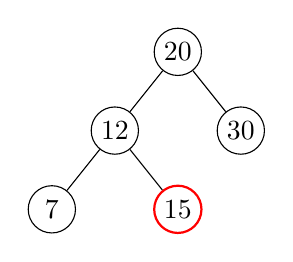
\begin{tikzpicture}[level distance=10mm, sibling distance=16mm,
    every node/.style={circle, draw, minimum size=6mm, inner sep=0pt}]
    \node {20}
        child {node {12}
            child {node {7}}
            child {node[draw=red, thick] {15}}
        }
        child {node {30}};
\end{tikzpicture}
\quad $\Longrightarrow$ \quad
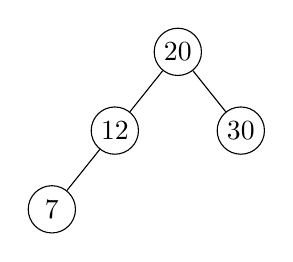
\begin{tikzpicture}[level distance=10mm, sibling distance=16mm,
    every node/.style={circle, draw, minimum size=6mm, inner sep=0pt}]
    \node {20}
        child {node {12}
            child {node {7}}
            child[missing] {}
        }
        child {node {30}};
\end{tikzpicture}
\end{center}

Find parent pointer ($12$'s right), assign \texttt{nullptr}, delete the node. If the leaf \emph{is} the root, the tree becomes empty.

\subsection*{Case 2: removing a node with one child}

\begin{center}
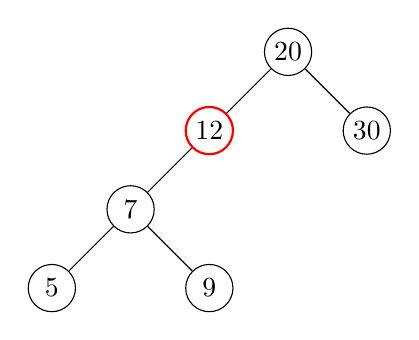
\begin{tikzpicture}[level distance=10mm, sibling distance=20mm,
    every node/.style={circle, draw, minimum size=6mm, inner sep=0pt}]
    \node {20}
        child {node[draw=red, thick] {12}
            child {node {7}
                child {node {5}}
                child {node {9}}
            }
            child[missing] {}
        }
        child {node {30}};
\end{tikzpicture}
\quad $\Longrightarrow$ \quad
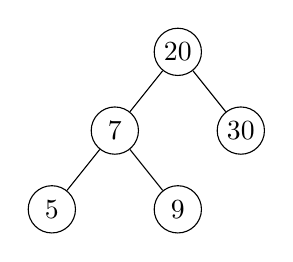
\begin{tikzpicture}[level distance=10mm, sibling distance=16mm,
    every node/.style={circle, draw, minimum size=6mm, inner sep=0pt}]
    \node {20}
        child {node {7}
            child {node {5}}
            child {node {9}}
        }
        child {node {30}};
\end{tikzpicture}
\end{center}

The parent of $12$ (here, $20$) re-points its left child to $12$'s only child, $7$. The whole subtree below $7$ rides along untouched -- BST ordering is preserved because everything there was already $<12<20$, which still obeys the grandparent.

\subsection*{Case 3: removing a node with two children}

\begin{center}
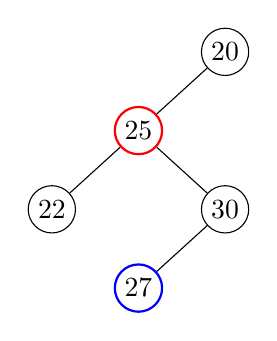
\begin{tikzpicture}[level distance=10mm, sibling distance=22mm,
    every node/.style={circle, draw, minimum size=6mm, inner sep=0pt}]
    \node {20}
        child {node[draw=red, thick] {25}
            child {node {22}}
            child {node {30}
                child {node[draw=blue, thick] {27}} child[missing] {}
            }
        }
        child[missing] {};
\end{tikzpicture}
\quad $\Longrightarrow$ \quad
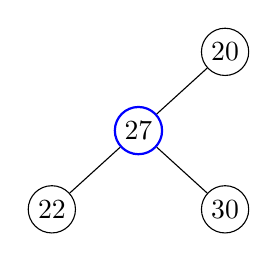
\begin{tikzpicture}[level distance=10mm, sibling distance=22mm,
    every node/.style={circle, draw, minimum size=6mm, inner sep=0pt}]
    \node {20}
        child {node[draw=blue, thick] {27}
            child {node {22}}
            child {node {30}}
        }
        child[missing] {};
\end{tikzpicture}
\end{center}

We wanted to delete $25$. The successor of $25$ is $27$ -- leftmost node of $25$'s right subtree (walk right once to $30$, then left as far as possible, arriving at $27$). Copy $27$'s key into $25$'s node, then delete $27$ from the right subtree. Because $27$ was the \emph{leftmost}, it has no left child, so that recursive delete is a case-1 or case-2 cleanup.

\subsection*{C++ implementation}

The reference-to-pointer pattern from insertion pays off again. Each subtree root is passed as \texttt{TreeNode*\&}, so re-assignment rewires the parent's child slot in place.

\begin{lstlisting}
void removeMin(TreeNode<int>*& root) {
    // Precondition: root != nullptr.
    // Deletes the leftmost node and splices in its right child.
    if (root->left == nullptr) {
        TreeNode<int>* old = root;
        root = root->right;
        delete old;
        return;
    }
    removeMin(root->left);
}

bool bstRemove(TreeNode<int>*& root, int key) {
    if (root == nullptr) return false;

    if (key < root->data) return bstRemove(root->left, key);
    if (key > root->data) return bstRemove(root->right, key);

    // Found it.
    if (root->left == nullptr) {
        TreeNode<int>* old = root;
        root = root->right;          // Cases 1 and 2 (right-only or leaf).
        delete old;
    } else if (root->right == nullptr) {
        TreeNode<int>* old = root;
        root = root->left;           // Case 2 (left-only).
        delete old;
    } else {
        // Case 3: copy successor, then delete it from the right subtree.
        TreeNode<int>* succ = root->right;
        while (succ->left != nullptr) succ = succ->left;
        root->data = succ->data;
        removeMin(root->right);
    }
    return true;
}
\end{lstlisting}

\begin{notebox}
Splitting out \texttt{removeMin} is a common refactor -- it's exactly the case-3 cleanup step and it's cheaper than a second full \texttt{bstRemove} call (no comparisons, just a straight walk left). The textbook pseudocode inlines a recursive call to \texttt{BSTRemove}; both are correct.
\end{notebox}

\subsection*{Iterative bookkeeping: the parent pointer}

The recursive version above hides the parent. An iterative version has to track it explicitly:

\begin{lstlisting}
// cur walks down. par trails one step behind so we can rewrite par's child.
TreeNode<int>* par = nullptr;
TreeNode<int>* cur = root;
while (cur != nullptr && cur->data != key) {
    par = cur;
    cur = (key < cur->data) ? cur->left : cur->right;
}
if (cur == nullptr) return;  // Not found.
// ... case split on cur->left / cur->right, rewrite par->left or par->right.
\end{lstlisting}

This is what the textbook pseudocode does. The recursive \texttt{TreeNode*\&} trick is cleaner in C++, but the iterative \texttt{par}/\texttt{cur} pair is universal.

\subsection*{Cost}

\begin{center}
\begin{tabular}{lll}
Operation & Best / balanced & Worst (skewed) \\
\hline
Search to find $X$       & $O(\log N)$ & $O(N)$ \\
Find successor (case 3)  & $O(\log N)$ & $O(N)$ \\
Pointer rewrite          & $O(1)$      & $O(1)$ \\
\hline
\textbf{Total}           & $O(\log N)$ & $O(N)$ \\
\end{tabular}
\end{center}

Space is $O(1)$ for the iterative version, $O(h)$ stack for the recursive one. Removal inherits the same balanced-vs-skewed story as search and insert -- the tree's shape dominates everything.

\begin{warnbox}
Don't free \texttt{cur} before you finish reading \texttt{cur->data}, \texttt{cur->left}, and \texttt{cur->right}. A very common bug: \texttt{delete cur; root = cur->right;} reads freed memory. Stash pointers first, delete last.
\end{warnbox}

\begin{ideabox}
Insertion only adds leaves; removal can touch anywhere. That asymmetry is why a naive BST degrades under churn: if your workload is insert-heavy with sorted-ish input, the tree grows one-sided and never self-corrects. AVL and red-black trees in later sections exist precisely to guarantee $O(\log N)$ \emph{after} arbitrary sequences of inserts and removes.
\end{ideabox}

\section{6.7 BST Traversals}

A BST stores keys \emph{structurally} sorted -- the ordering invariant means a simple recursive walk can visit every node in sorted order. That walk is called an \textbf{in-order traversal}, and it's the single biggest reason BSTs earn their keep: you get $O(n)$ sorted output for free, without ever calling a comparison-based sort.

\begin{defnbox}[Tree traversal]
A \emph{traversal} visits every node in the tree exactly once, performing some operation (print, count, collect into a list, transform into another structure) on each node. Binary trees have three classical traversal orders, distinguished by when the \emph{current} node is visited relative to its two subtrees.
\end{defnbox}

\subsection*{Three orders, one skeleton}

All three traversals share the same shape. They differ only in where the ``visit current'' step lives:

\begin{center}
\begin{tabular}{lll}
\textbf{Order}   & \textbf{Pattern} & \textbf{On a BST, this prints\dots} \\
\hline
Pre-order        & Cur, Left, Right & keys in root-first order (serialization) \\
\textbf{In-order} & \textbf{Left, Cur, Right} & \textbf{keys in ascending sorted order} \\
Post-order       & Left, Right, Cur & keys in leaf-first order (safe for delete) \\
\end{tabular}
\end{center}

In-order is what the chapter focuses on. The other two matter later: pre-order is how you serialize or copy a tree, post-order is the deletion order (free the children before the parent).

\subsection*{In-order traversal: the algorithm}

\begin{lstlisting}
template <typename T>
void bstPrintInorder(const TreeNode<T>* node) {
    if (node == nullptr) return;
    bstPrintInorder(node->left);   // everything smaller than node
    std::cout << node->data << ' '; // node itself
    bstPrintInorder(node->right);  // everything larger than node
}
\end{lstlisting}

Three lines of logic, after the base case. The BST ordering invariant does the rest: everything in the left subtree is $<$ \texttt{node->data}, everything in the right is $>$, so printing them in the order left-cur-right yields ascending sequence.

\subsection*{Walk-through}

Trace the in-order traversal of:

\begin{center}
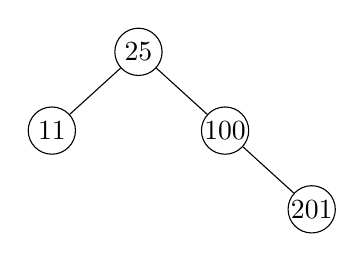
\begin{tikzpicture}[level distance=10mm, sibling distance=22mm,
    every node/.style={circle, draw, minimum size=6mm, inner sep=0pt}]
    \node {25}
        child {node {11}}
        child {node {100}
            child[missing] {}
            child {node {201}}
        };
\end{tikzpicture}
\end{center}

\begin{enumerate}[leftmargin=*]
    \item Call on 25. Descend into left child $\Rightarrow$ call on 11.
    \item Call on 11. Left is null $\Rightarrow$ return immediately. Print \textbf{11}. Right is null $\Rightarrow$ return.
    \item Back at 25. Left finished. Print \textbf{25}. Descend into right child $\Rightarrow$ call on 100.
    \item Call on 100. Left is null. Print \textbf{100}. Descend into right $\Rightarrow$ call on 201.
    \item Call on 201. Both children null. Print \textbf{201}. Return.
\end{enumerate}

Output: \texttt{11 25 100 201}. Sorted, as promised.

\begin{ideabox}
Notice that the nodes are printed \emph{not} in the order the recursion discovers them. The algorithm discovers 25, then 11, then jumps to 100, then 201 -- but the \emph{print} happens only after both children have been fully handled on the left side. The call stack is what holds the out-of-order positions until it's their turn.
\end{ideabox}

\subsection*{Why it works: a one-line proof}

Induction on tree height. A null tree prints nothing -- trivially sorted. Suppose in-order prints every smaller tree in sorted order. For the current tree: by the BST invariant, left-subtree keys are all $<$ \texttt{node->data} and right-subtree keys are all $>$. By the induction hypothesis, the left-subtree call prints its contents in sorted order, followed by \texttt{node->data}, followed by the right-subtree contents in sorted order. Concatenated, that's the whole tree in sorted order.

\subsection*{Cost}

\begin{center}
\begin{tabular}{ll}
Time  & $O(n)$ -- each node is visited exactly once \\
Space & $O(h)$ recursion stack, where $h$ is tree height \\
\end{tabular}
\end{center}

The time bound is tight and independent of shape -- a skewed tree still traverses in $O(n)$, because you still visit every node once. The \emph{space} bound is where shape matters: a balanced tree uses $O(\log n)$ stack, a degenerate chain uses $O(n)$.

\begin{notebox}
Since in-order on a BST is sorted, you can implement a ``sort an array via BST'' algorithm: insert every element, then in-order traverse. Cost: $O(n \log n)$ average if the input is random, $O(n^2)$ worst case if the input is already sorted (insert degrades). This is how tree sort works, and it's why self-balancing trees (AVL, red-black) exist -- they make tree sort reliably $O(n \log n)$.
\end{notebox}

\subsection*{Pre-order and post-order: the sketches}

\begin{lstlisting}
template <typename T>
void bstPrintPreorder(const TreeNode<T>* node) {
    if (node == nullptr) return;
    std::cout << node->data << ' ';
    bstPrintPreorder(node->left);
    bstPrintPreorder(node->right);
}

template <typename T>
void bstDestroyPostorder(TreeNode<T>* node) {
    if (node == nullptr) return;
    bstDestroyPostorder(node->left);
    bstDestroyPostorder(node->right);
    delete node;                 // safe: children are already gone
}
\end{lstlisting}

Pre-order on the example tree above prints \texttt{25 11 100 201}; post-order prints \texttt{11 201 100 25}. Same nodes, different orders, same $O(n)$ cost.

\begin{warnbox}
The in-order output being sorted is a property of \textbf{BSTs specifically}. For a generic binary tree with no ordering invariant, in-order just gives ``left-cur-right'' in structural order -- no sortedness. If you find yourself relying on sorted output from in-order, make sure the tree you're walking is actually a BST.
\end{warnbox}

\section{6.8 BST Height and Insertion Order}

This is the section where the textbook cashes in on all the caveats. We've said ``$O(\log n)$ in the balanced case, $O(n)$ in the worst case'' for every operation. Now we confront what actually \emph{causes} the worst case, and measure the shape of the tree we end up with.

\subsection*{Bounds on height}

For an $N$-node binary tree, the height $h$ is bounded by:
\[
\lfloor \log_2 N \rfloor \;\le\; h \;\le\; N - 1
\]

\begin{itemize}[leftmargin=*]
    \item \textbf{Minimum:} $h = \lfloor \log_2 N \rfloor$, achieved when every level is full except possibly the last. This is a \emph{complete} binary tree.
    \item \textbf{Maximum:} $h = N - 1$, achieved when every node has at most one child. This is a \emph{degenerate} tree (a glorified linked list).
\end{itemize}

Search, insertion, and removal all cost $O(h)$. So the difference between $h = \log_2 N$ and $h = N-1$ is the difference between a responsive tree on millions of keys and something that stalls.

\begin{center}
\small
\begin{tabular}{rll}
$N$ & $\log_2 N$ & $N - 1$ \\
\hline
$10$    & $\approx 3$   & $9$ \\
$1\,000$   & $\approx 10$  & $999$ \\
$10^6$  & $\approx 20$  & $999\,999$ \\
\end{tabular}
\end{center}

A million-node balanced BST finds a key in 20 comparisons. A degenerate one takes a million.

\subsection*{What controls the shape? Insertion order.}

A raw (non-self-balancing) BST has no shape-correcting logic: it just drops new keys wherever the search path leads. So the tree that results from inserting a sequence is \emph{entirely} determined by that sequence.

\begin{defnbox}[The insertion-order rule]
\begin{itemize}[leftmargin=*]
    \item \textbf{Random-order inserts:} expected height is $O(\log N)$. In practice the tree stays close to balanced.
    \item \textbf{Sorted (or reverse-sorted) inserts:} height is exactly $N - 1$. Each new key becomes the rightmost (or leftmost) node, forming a chain.
    \item \textbf{Nearly-sorted inserts:} height is $\Theta(N)$. You don't need perfectly sorted input to get worst-case behavior -- ``mostly sorted'' is already disastrous.
\end{itemize}
\end{defnbox}

\subsection*{Example: sorted vs. random}

Insert $[1, 2, 3, 4, 5]$ in that order into an empty BST:

\begin{center}
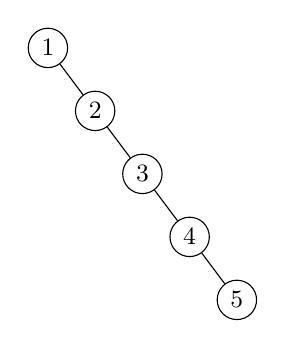
\begin{tikzpicture}[level distance=8mm, sibling distance=12mm,
    every node/.style={circle, draw, minimum size=5mm, inner sep=0pt, font=\small}]
    \node {1}
        child[missing] {}
        child {node {2}
            child[missing] {}
            child {node {3}
                child[missing] {}
                child {node {4}
                    child[missing] {}
                    child {node {5}}
                }
            }
        };
\end{tikzpicture}
\end{center}

Height $= 4 = N - 1$. Completely right-skewed. Search for $5$ takes 5 comparisons.

Insert the same keys in a randomized order, say $[3, 1, 4, 5, 2]$:

\begin{center}
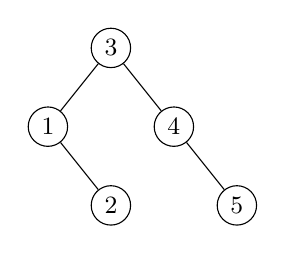
\begin{tikzpicture}[level distance=10mm, sibling distance=16mm,
    every node/.style={circle, draw, minimum size=5mm, inner sep=0pt, font=\small}]
    \node {3}
        child {node {1}
            child[missing] {}
            child {node {2}}
        }
        child {node {4}
            child[missing] {}
            child {node {5}}
        };
\end{tikzpicture}
\end{center}

Height $= 2 \approx \lfloor \log_2 5 \rfloor$. Search for $5$ takes 3 comparisons. \emph{Same keys, same BST data structure, wildly different performance.}

\begin{ideabox}
This is the central flaw of the raw BST: performance depends on \emph{the order keys arrived}, not on the keys themselves. A dataset you'd consider ``clean'' -- sorted by user ID, by timestamp, by anything -- is exactly the \emph{worst} input for a raw BST. Real-world data is rarely adversarial but frequently sorted-ish.
\end{ideabox}

\subsection*{Computing the height: \texttt{bstGetHeight}}

Height is defined recursively -- perfect match for a recursive traversal:

\begin{lstlisting}
template <typename T>
int bstGetHeight(const TreeNode<T>* node) {
    if (node == nullptr) return -1;   // null subtree has height -1
    int lh = bstGetHeight(node->left);
    int rh = bstGetHeight(node->right);
    return 1 + std::max(lh, rh);
}
\end{lstlisting}

The $-1$ base case is the trick: it makes a single-node tree (both children null) return $1 + \max(-1, -1) = 0$, which matches the definition ``a single-node tree has height 0.''

\subsection*{Walk-through of \texttt{bstGetHeight}}

For the tree rooted at $20$ with the shape $(20 \;\; (18 \;(12\;(-,14),-)) \;\; 30)$:

\begin{enumerate}[leftmargin=*]
    \item \texttt{bstGetHeight(20)} recurses left to $18$.
    \item \texttt{bstGetHeight(18)} recurses left to $12$, which recurses left to \texttt{null} $\rightarrow -1$.
    \item \texttt{bstGetHeight(12)} now recurses right to $14$, which returns $1 + \max(-1, -1) = 0$.
    \item \texttt{bstGetHeight(12)} returns $1 + \max(-1, 0) = 1$.
    \item \texttt{bstGetHeight(18)} then recurses right to \texttt{null} $\rightarrow -1$. Returns $1 + \max(1, -1) = 2$.
    \item Back at $20$, the right child $30$ is a leaf and returns $0$. The root returns $1 + \max(2, 0) = 3$.
\end{enumerate}

Tree height $= 3$. Cost of \texttt{bstGetHeight}: visits every node once, so $O(n)$ time and $O(h)$ stack.

\subsection*{Cost recap with height in the driver's seat}

\begin{center}
\begin{tabular}{lll}
Operation & Cost & Explanation \\
\hline
\texttt{search}, \texttt{insert}, \texttt{remove} & $O(h)$ & one walk down the tree \\
\texttt{inorder traversal}         & $O(n)$ & visit every node \\
\texttt{bstGetHeight}              & $O(n)$ & visit every node \\
\end{tabular}
\end{center}

For a tree where $h = \log_2 n$, the per-op cost is logarithmic. For $h = n - 1$, it's linear. \emph{Every} BST bound funnels through $h$.

\begin{notebox}
If you control the insertion order and the keys are known up front, you can shuffle before inserting. That's a quick fix and often good enough. For streaming inserts or adversarial input, you need a tree that re-balances itself -- AVL and red-black trees (ch.~9) do exactly that, paying a constant-factor per-op cost to guarantee $h = O(\log n)$ forever.
\end{notebox}

\begin{warnbox}
Don't confuse ``height'' with ``depth.'' Height is measured \emph{up from the leaves} to a node (or equivalently, the deepest path in that subtree). Depth is measured \emph{down from the root}. A tree's height equals the maximum depth of any node, but don't conflate the two when computing either one. The algorithm above computes height, not depth.
\end{warnbox}

\begin{notebox}[Random insertion gives $O(\log n)$ height in expectation]
The ``height = $n - 1$ disaster'' above only happens with
\emph{adversarial} insertion order (sorted, reverse-sorted, etc).
What about random order?

\textbf{CLRS Theorem 12.4.} A randomly built BST on $n$ distinct
keys --- one constructed by inserting the keys in a uniformly random
permutation into an initially empty tree --- has expected height
$O(\log n)$.

The proof parallels randomized quicksort: the random rank of the
root key splits the remaining keys into two roughly-balanced
subproblems on average, and the recursion bottoms out at depth
$O(\log n)$ with high probability.

\textbf{Practical implication.} Plain BSTs with random or
adversary-free input behave like balanced trees on average. This is
why a vanilla BST survives in real codebases: the typical case is
already $O(\log n)$. The reason production systems still reach for
red-black trees (ch.~9) is \emph{worst-case guarantees} --- a hard
$O(\log n)$ bound on every single operation, plus immunity to
adversarial input that forces the pathological shape.

This is the same pattern as the universal-hashing story from
\textsection 5.7: random structure makes the average case good;
defending the worst case requires more (rotations for trees,
universal hashing for tables).
\end{notebox}

\begin{defnbox}[Rotation: the local fix-up that preserves the BST invariant]
A \emph{rotation} reorganizes three pointers so that one node moves
up and another moves down. It is local: only the two nodes and
their immediate subtrees are touched. It is invariant-preserving:
the BST in-order key ordering is identical before and after.

A \emph{left-rotation around $y$}, when $y$'s right child is $x$:
\begin{verbatim}
       y                       x
      / \                     / \
     A   x        ===>       y   C
        / \                 / \
       B   C               A   B
\end{verbatim}
Read both trees in-order: \texttt{A y B x C}. Same sequence both
times. The keys haven't moved relative to each other --- only their
position in the tree's hierarchy has.

\textbf{Why this matters.} ch.~9 (AVL + red-black) keeps the tree
balanced by performing a small number of rotations after every
insert and remove. The result: $h$ stays $O(\log n)$ regardless of
input order, so every operation in the chapter you just read keeps
its best-case cost guaranteed instead of just on average. The BST
algorithms don't change; the maintenance code does.
\end{defnbox}

\section{6.9 BST Parent Pointers}

Up to this section, our \texttt{TreeNode} has held only \texttt{data}, \texttt{left}, and \texttt{right}. Every algorithm has propagated ``who is my parent?'' information down through recursion or through a trailing \texttt{par} pointer in iterative code. That works, but it means \emph{going up the tree always requires re-descending from the root.} Self-balancing trees (AVL, red-black) rebalance after a modification, and the rebalancing always starts at the modified node and walks \emph{upward} -- they need $O(1)$ access to the parent.

The fix is a third pointer per node.

\begin{defnbox}[Parent pointer]
Each \texttt{TreeNode} gets an additional field \texttt{parent} -- a pointer to the node whose \texttt{left} or \texttt{right} points to this one. The root has \texttt{parent = nullptr}. The invariant to maintain: for every non-null node $n$, \texttt{n->parent->left == n} \textbf{or} \texttt{n->parent->right == n}, and the root has no parent.
\end{defnbox}

\begin{lstlisting}
template <typename T>
struct TreeNode {
    T          data;
    TreeNode*  left   = nullptr;
    TreeNode*  right  = nullptr;
    TreeNode*  parent = nullptr;   // new
};
\end{lstlisting}

\subsection*{What the extra pointer buys you}

\begin{itemize}[leftmargin=*]
    \item $O(1)$ parent lookup from any node.
    \item $O(1)$ sibling lookup (if \texttt{node == node->parent->left} the sibling is \texttt{node->parent->right}, else \texttt{node->parent->left}).
    \item Walking upward until a rotation point is found -- essential for AVL's retrace step and red-black's fix-up.
    \item Iterator-style traversals (give me the next in-order node) can be implemented without a stack.
\end{itemize}

The cost: one extra pointer per node (same memory cost as a doubly-linked list over a singly-linked list), and \emph{every} insertion and removal must now maintain the parent-pointer invariant.

\subsection*{Insert with parent wiring}

The search walk is unchanged. The difference is that when we finally attach the new node, we wire up \texttt{new->parent} to the node we attached below:

\begin{lstlisting}
template <typename T>
void bstInsert(TreeNode<T>*& root, TreeNode<T>* node) {
    node->left = node->right = node->parent = nullptr;

    if (root == nullptr) { root = node; return; }

    TreeNode<T>* cur = root;
    while (true) {
        if (node->data < cur->data) {
            if (cur->left == nullptr) {
                cur->left    = node;
                node->parent = cur;     // wire the back-pointer
                return;
            }
            cur = cur->left;
        } else {
            if (cur->right == nullptr) {
                cur->right   = node;
                node->parent = cur;     // wire the back-pointer
                return;
            }
            cur = cur->right;
        }
    }
}
\end{lstlisting}

\subsection*{A tiny helper: \texttt{bstReplaceChild}}

Removal with parent pointers becomes much cleaner if we factor out the ``swap this child out for that one'' operation. Because any node that isn't the root knows its parent, we can write:

\begin{lstlisting}
template <typename T>
bool bstReplaceChild(TreeNode<T>* parent,
                     TreeNode<T>* currentChild,
                     TreeNode<T>* newChild) {
    if (parent->left != currentChild && parent->right != currentChild)
        return false;

    if (parent->left == currentChild) parent->left = newChild;
    else                              parent->right = newChild;

    if (newChild != nullptr) newChild->parent = parent;
    return true;
}
\end{lstlisting}

This helper guarantees two things at once: the parent's \texttt{left}/\texttt{right} slot gets the new child, \emph{and} the new child's \texttt{parent} back-pointer gets updated. Without this helper you will eventually write code that updates one direction and forgets the other -- that's the single most common parent-pointer bug.

\subsection*{Removal, redone with parent pointers}

Splitting removal into two functions is idiomatic once you have parent pointers: the outer \texttt{bstRemoveKey} finds the node by key, the inner \texttt{bstRemoveNode} removes a known node. The inner version is the one that AVL and red-black trees will override to hook in rebalancing.

\begin{lstlisting}
template <typename T>
void bstRemoveKey(TreeNode<T>*& root, const T& key) {
    TreeNode<T>* node = bstSearch(root, key);
    bstRemoveNode(root, node);
}

template <typename T>
void bstRemoveNode(TreeNode<T>*& root, TreeNode<T>* node) {
    if (node == nullptr) return;

    // Case 1: two children -- copy successor, recurse to remove it.
    if (node->left != nullptr && node->right != nullptr) {
        TreeNode<T>* succ = node->right;
        while (succ->left != nullptr) succ = succ->left;
        node->data = succ->data;
        bstRemoveNode(root, succ);
        return;
    }

    // One or zero children from here on.
    TreeNode<T>* only = (node->left != nullptr) ? node->left : node->right;

    // Case 2: the node is the root.
    if (node == root) {
        root = only;
        if (root != nullptr) root->parent = nullptr;
    }
    // Case 3 & 4: splice the only (possibly-null) child in below node->parent.
    else {
        bstReplaceChild(node->parent, node, only);
    }

    delete node;
}
\end{lstlisting}

Compare this to the reference-to-pointer version from 6.6. Both are correct; the parent-pointer version has four clean cases that mirror the textbook's breakdown, and the \texttt{bstReplaceChild} helper keeps the back-pointer invariant airtight.

\subsection*{Worked case analysis}

\begin{center}
\begin{tabular}{lll}
Case & Condition & Action \\
\hline
1 & two children       & Copy successor's data, recurse on successor \\
2 & is the root        & Promote lone child (or null) as the new root \\
3 & only left child    & \texttt{bstReplaceChild(parent, node, node->left)} \\
4 & only right / none  & \texttt{bstReplaceChild(parent, node, node->right)} \\
\end{tabular}
\end{center}

Case 1 recursing into the successor is safe: the successor has at most one child (it was the leftmost of the right subtree), so the recursive call falls into case 2, 3, or 4.

\begin{ideabox}
The parent pointer is a trade: one extra pointer per node and careful wiring on every mutation, in exchange for $O(1)$ upward traversal. For a raw BST that only does search/insert/remove, it's not worth it -- descent-based code gets the same information from the recursion stack. For a self-balancing tree, it's \emph{essential} -- AVL's retrace walks upward from the modified leaf, and red-black's fix-up walks upward from the newly-inserted node looking for violated constraints.
\end{ideabox}

\subsection*{The wiring traps}

\begin{warnbox}
The invariant ``every non-root node has a parent whose child-slot points back at it'' is easy to state but easy to break:
\begin{itemize}[leftmargin=*]
    \item Forgetting to set \texttt{new->parent} when inserting.
    \item Forgetting to \texttt{null} the old node's parent pointer when promoting a child to root.
    \item Copying nodes (by value!) in case 1 -- the successor's \emph{data} is copied, not the node. If you accidentally re-wire around the successor's node instead, you leave dangling parent pointers.
    \item \texttt{bstReplaceChild} with \texttt{newChild = nullptr} is legal (that's how leaves are removed), but you must skip the \texttt{newChild->parent = parent} assignment in that case.
\end{itemize}
Using \texttt{bstReplaceChild} everywhere instead of hand-rolling the assignment eliminates most of these bugs.
\end{warnbox}

\section{6.10 Recursive BST Implementations (No Parent Pointers)}

This section closes the chapter by revisiting the core BST operations -- search, find-parent, insert, remove -- as \emph{recursive} algorithms on a plain BST without parent pointers. The point isn't to pick a winner between iterative and recursive: both are correct and produce identical trees. The point is to see how the tree-shaped data structure wants to be written tree-shaped, and to recognize the patterns you'll need again for AVL, red-black, tries, and every other hierarchical structure in your future.

\begin{ideabox}
The recursion mirrors the structure of the data. Every non-trivial BST problem has the shape ``do something at the root, recurse into the appropriate subtree.'' That symmetry is why recursion often produces the shortest, clearest code for trees. The recursion stack plays the role of the \texttt{parent} pointer chain from section 6.9 -- going ``up'' is just returning from a recursive call.
\end{ideabox}

\subsection*{Recursive search}

The recursive version of search is almost a direct transcription of the ordering invariant:

\begin{lstlisting}
template <typename T>
const TreeNode<T>* bstSearch(const TreeNode<T>* node, const T& key) {
    if (node == nullptr)       return nullptr;       // base: not found
    if (key == node->data)     return node;          // base: found
    if (key < node->data)      return bstSearch(node->left,  key);
    return                            bstSearch(node->right, key);
}
\end{lstlisting}

Two base cases, two recursive cases. Each call does $O(1)$ work and chooses exactly one child, so the total cost is $O(h)$ -- same as iterative. The difference is purely syntactic. The recursive version uses $O(h)$ stack rather than $O(1)$, so on a pathological chain you can blow the stack -- but that's the same input that would make any BST operation slow, so it's rarely the binding concern.

\begin{notebox}
Each of the three recursive calls is in \emph{tail position} (the last thing the function does). A smart compiler can optimize this to a loop (tail-call elimination), giving you iterative performance from recursive code. GCC and Clang do this reliably at \texttt{-O2}. You don't have to manually iterativize search for perf reasons -- write it however is clearest, measure if you care.
\end{notebox}

\subsection*{Recursive find-parent (without parent pointers)}

Section 6.9 added a \texttt{parent} pointer to each node to make ``who is my parent?'' a $O(1)$ lookup. Without that field, you have to walk from the root again. The algorithm is structurally identical to \texttt{bstSearch} -- just with a different base case.

\begin{lstlisting}
template <typename T>
TreeNode<T>* bstGetParent(TreeNode<T>* subtreeRoot, const TreeNode<T>* node) {
    if (subtreeRoot == nullptr) return nullptr;
    if (subtreeRoot->left == node || subtreeRoot->right == node)
        return subtreeRoot;                          // base: found the parent
    if (node->data < subtreeRoot->data)
        return bstGetParent(subtreeRoot->left,  node);
    return bstGetParent(subtreeRoot->right, node);
}
\end{lstlisting}

Notice the base case compares \emph{pointers}, not keys: \texttt{subtreeRoot->left == node}. Key comparison would be wrong if the tree contained duplicates. Pointer comparison asks ``is the node I'm looking for literally this one's child?''

Cost: $O(h)$. Same as search, because the decision of which subtree to recurse into is made with the same key comparison.

\subsection*{Recursive insertion}

The recursive insert descends until it finds a null child slot, then attaches the new node:

\begin{lstlisting}
template <typename T>
void bstInsertRec(TreeNode<T>* parent, TreeNode<T>* nodeToInsert) {
    if (nodeToInsert->data < parent->data) {
        if (parent->left == nullptr) parent->left = nodeToInsert;
        else bstInsertRec(parent->left, nodeToInsert);
    } else {
        if (parent->right == nullptr) parent->right = nodeToInsert;
        else bstInsertRec(parent->right, nodeToInsert);
    }
}

template <typename T>
void bstInsert(TreeNode<T>*& root, TreeNode<T>* node) {
    if (root == nullptr) root = node;
    else                 bstInsertRec(root, node);
}
\end{lstlisting}

Compare this with the reference-to-pointer version from 6.5 (\texttt{TreeNode*\&} everywhere). That version is arguably more elegant -- it handles the empty-tree case without a wrapper, because the reference to the caller's pointer \emph{is} where we write. The \texttt{parent}-passing version here has to special-case the empty root in the outer wrapper. Both are valid; the \texttt{TreeNode*\&} version is tighter C++, the \texttt{parent}-passing version translates more directly to languages without reference semantics (Java, Python, Go).

\subsection*{Recursive removal}

Removal combines \texttt{bstSearch} (to find the node) and \texttt{bstGetParent} (to find its parent) and then applies the four cases from section 6.6:

\begin{lstlisting}
template <typename T>
bool bstRemoveNode(TreeNode<T>*& root,
                   TreeNode<T>* parent,
                   TreeNode<T>* node) {
    if (node == nullptr) return false;

    // Case 1: two children. Find successor + its parent, copy, recurse.
    if (node->left != nullptr && node->right != nullptr) {
        TreeNode<T>* succ       = node->right;
        TreeNode<T>* succParent = node;
        while (succ->left != nullptr) {
            succParent = succ;
            succ       = succ->left;
        }
        node->data = succ->data;
        return bstRemoveNode(root, succParent, succ);
    }

    TreeNode<T>* only = (node->left != nullptr) ? node->left : node->right;

    // Case 2: node is the root.
    if (node == root) {
        root = only;
    }
    // Cases 3 & 4: splice below parent.
    else if (parent->left == node) parent->left  = only;
    else                           parent->right = only;

    delete node;
    return true;
}

template <typename T>
bool bstRemove(TreeNode<T>*& root, const T& key) {
    TreeNode<T>* node   = const_cast<TreeNode<T>*>(bstSearch(root, key));
    TreeNode<T>* parent = bstGetParent(root, node);
    return bstRemoveNode(root, parent, node);
}
\end{lstlisting}

This is the same four-case removal as before. The key implementation difference is that \texttt{succParent} is tracked explicitly during the successor walk -- since we have no parent pointers, we can't ask the successor for its parent, so we maintain the trailing pointer manually (exactly the \texttt{par}/\texttt{cur} trick from iterative search).

\subsection*{Comparison: three ways to remove a node}

\begin{center}
\begin{tabular}{lll}
Version & Extra state per node & Cost of finding parent \\
\hline
\texttt{TreeNode*\&} reference (6.6) & none & free (held in the recursion) \\
parent pointers (6.9)                 & +1 pointer & $O(1)$ \\
plain recursive + \texttt{bstGetParent} (6.10) & none & $O(h)$ (re-search) \\
\end{tabular}
\end{center}

The recursive version with \texttt{bstGetParent} is the slowest of the three for removal -- you pay $O(h)$ once for search, then again for \texttt{bstGetParent}. It's still $O(h)$ total asymptotically, but the constant doubles. The \texttt{TreeNode*\&} version is the tightest for a raw BST. The parent-pointer version is what real libraries use when they're building AVL or red-black on top.

\begin{ideabox}
The three implementations are \emph{equivalent in behavior} -- they produce the same trees from the same operations. They differ only in how parent information is retrieved: implicitly via the recursion stack, explicitly via a stored pointer, or on demand by re-searching. Choose based on what else the structure needs. A raw BST: reference-to-pointer. A self-balancing tree: parent pointers. A teaching example where you want two operations to feel symmetric: plain recursion with \texttt{bstGetParent}.
\end{ideabox}

\begin{warnbox}
Watch the succession walk in case 1 carefully. The \texttt{while (succ->left != nullptr)} loop walks \emph{through} the successor's ancestors, updating \texttt{succParent} each step. If you initialize \texttt{succParent = nullptr} and forget that \texttt{node->right} itself might be the successor (when its left is null), you'll end up with \texttt{succParent = nullptr} at case-1's recursive call, and the recursion will mis-handle the splice. Initialize \texttt{succParent = node}.
\end{warnbox}

\begin{notebox}
Chapter 6 ends here. The next chapters extend these foundations to self-balancing trees (AVL and red-black), heaps (array-backed complete trees with the partial-order invariant), and general trees / tries. Everything we've built -- recursion on subtrees, the left-root-right pattern, the four-case removal -- will reappear, sometimes unchanged, sometimes augmented with rebalancing rotations. The shape is stable; the invariants get stricter.
\end{notebox}

\section*{What this connects to}

\begin{notebox}[Forward links to later chapters]
\begin{itemize}
    \item \textbf{Chapter 9 (AVL, red-black).} These make the BST
    $O(\log n)$ guarantee tight instead of best-case. Every rotation
    preserves the BST invariant from this chapter; only the balance
    invariant is new. If BST insert/remove is shaky, AVL won't land.
    \item \textbf{Optional ch.~11 (B-trees / 2-3-4 trees).} Generalizes
    ``one key per node, two children'' to ``multiple keys, multiple
    children.'' Used by on-disk databases and filesystems.
    \item \textbf{\texttt{std::map} / \texttt{std::set}.} Both are
    red-black trees under the hood. Choosing between them and their
    \texttt{unordered\_} hash-based cousins is the ADT-vs-data-structure
    decision from ch.~3, now grounded in a real cost model.
    \item \textbf{Heaps and priority queues.} Heaps are another
    hierarchical structure, but instead of BST's key-ordering invariant
    they use a \emph{partial-order} (parent $\leq$ child) invariant.
    Same node + children idea, different constraint.
    \item \textbf{Graphs (opt.\ ch.~10).} Graph traversal generalizes
    tree traversal: a tree is a graph without cycles. BFS and DFS on
    graphs reuse the queue / stack idioms from ch.~4 and the recursion
    pattern from here.
\end{itemize}
\end{notebox}

\textbf{Companion materials.} Compact notes:
\texttt{chapters/ch\_6/notes.tex}. Practice prompts (problem $\to$
pseudocode $\to$ C++): \texttt{chapters/ch\_6/practice.md}.

\end{document}
